% Co-LIC2: Cooperative Multi-Node Photo-Realistic Gaussian SLAM
%    with QoS-Aware Multi-Stream Wireless Protocol
% MobiCom submission template (ACM acmart, sigconf)
% Compile: pdflatex main && bibtex main && pdflatex main && pdflatex main
\documentclass[sigconf, 10pt, review, anonymous]{acmart}

%% Rights / conference metadata (placeholder for submission; replace on acceptance)
\setcopyright{none}
\acmConference[MobiCom '27]{The 33rd Annual International Conference on Mobile Computing and Networking}{2027}{TBD}
\acmYear{2027}
\acmDOI{XXXXXXX.XXXXXXX}
\acmISBN{978-1-4503-XXXX-X/27/XX}

%% Math and graphics
\usepackage{amsmath,amsfonts}
\usepackage{mathtools}
\usepackage{booktabs}
\usepackage{subcaption}
\usepackage{multirow}
%% Fix acmart + amssymb conflict for \Bbbk
\let\Bbbk\relax
\usepackage{amssymb}

%% Algorithms
\usepackage{algorithm}
\usepackage{algpseudocode}

%% TikZ for diagrams
\usepackage{tikz}
\usetikzlibrary{positioning,arrows.meta,calc,fit,shapes.geometric,backgrounds,decorations.pathreplacing,patterns}

%% Listings for code/format snippets
\usepackage{listings}
\usepackage{xcolor}

%% Custom commands
\newcommand{\SEthree}{SE(3)}
\newcommand{\Twb}{T_{W\leftarrow B}}
\newcommand{\GaussianMap}{\mathcal{G}}
\newcommand{\submap}{\mathcal{S}}
\newcommand{\Npv}{\text{NPV}}
\newcommand{\Bbudget}{B_{\text{budget}}}
\newcommand{\coap}{\texttt{CoAP} }
\newcommand{\dds}{\texttt{DDS} }
\newcommand{\grpc}{\texttt{gRPC} }

\begin{document}

\title{Co-LIC2: Cooperative Multi-Node Photo-Realistic Gaussian SLAM\\with QoS-Aware Multi-Stream Wireless Protocol}

\author{Anonymous Author 1}
\affiliation{%
  \institution{Anonymous Institution}
  \city{Anonymous City}
  \country{Anonymous Country}}
\email{anon1@example.com}

\author{Anonymous Author 2}
\affiliation{%
  \institution{Anonymous Institution}
  \city{Anonymous City}
  \country{Anonymous Country}}
\email{anon2@example.com}

\author{Anonymous Author 3}
\affiliation{%
  \institution{Anonymous Institution}
  \city{Anonymous City}
  \country{Anonymous Country}}
\email{anon3@example.com}

\renewcommand{\shortauthors}{Anonymous}

\begin{abstract}
We present Co-LIC2, a cooperative multi-node LiDAR-inertial-visual Gaussian
Splatting SLAM system in which multiple mobile platforms communicate over
bandwidth-limited, lossy wireless networks to jointly construct a single
globally consistent photo-realistic 3D map. Co-LIC2 makes three contributions to
the intersection of mobile computing and robotic perception. First, we design a
\textbf{QoS-aware multi-stream wireless protocol} that multiplexes four traffic
classes---real-time pose streams, bulk submap transfers, reference keyframes,
and control messages---with differentiated reliability, latency, and priority.
Second, we introduce a \textbf{submap-aware adaptive compression scheduler} that
jointly optimizes spherical-harmonics truncation, spatial quantization, and
entropy-coding level under a hard bandwidth budget while maximizing
view-dependent rendering quality through a novel Number-of-Gaussians-Per-View
(NPV) metric. Third, we propose a \textbf{hierarchical hybrid network
architecture} with dynamic cluster-head election, multi-hop submap routing, and
graceful degradation pathways that maintain map consistency under intermittent
connectivity, node churn, and total network partition. We provide a detailed
protocol specification, analytical bounds on bandwidth scalability and
end-to-end latency, and a failure-mode recovery analysis. Co-LIC2's
communication layer is designed for Wi-Fi~6/6E and 5G~NR deployments, supporting
2--32 heterogeneous nodes with per-node uplink as low as 3.2~Mbps and per-cluster
inter-node submap merge latency under 2~s.
\end{abstract}

\begin{CCSXML}
<ccs2012>
 <concept>
  <concept_id>10003033.10003079.10003083</concept_id>
  <concept_desc>Networks~Network protocol design</concept_desc>
  <concept_significance>500</concept_significance>
 </concept>
 <concept>
  <concept_id>10003033.10003079.10003082</concept_id>
  <concept_desc>Networks~Wireless access networks</concept_desc>
  <concept_significance>500</concept_significance>
 </concept>
 <concept>
  <concept_id>10003120.10003121.10003122</concept_id>
  <concept_desc>Computer systems organization~Embedded and cyber-physical systems</concept_desc>
  <concept_significance>300</concept_significance>
 </concept>
 <concept>
  <concept_id>10010147.10010178.10010187</concept_id>
  <concept_desc>Computing methodologies~Computer vision</concept_desc>
  <concept_significance>300</concept_significance>
 </concept>
</ccs2012>
\end{CCSXML}

\ccsdesc[500]{Networks~Network protocol design}
\ccsdesc[500]{Networks~Wireless access networks}
\ccsdesc[300]{Computer systems organization~Embedded and cyber-physical systems}
\ccsdesc[300]{Computing methodologies~Computer vision}

\keywords{collaborative SLAM, Gaussian splatting, wireless protocol design,
QoS-aware streaming, multi-agent systems, edge computing, bandwidth-efficient
map sharing, hierarchical network topology}

\maketitle

\section{Introduction}
% ============================================
% Section: Introduction (MobiCom-focused, wireless-centric)
% ============================================

Cooperative autonomous systems---from multi-robot construction teams to
UAV--UGV disaster-response squads---require a shared, up-to-date 3D model of
their environment to plan, navigate, and coordinate. Recent advances in 3D
Gaussian Splatting (3DGS)~\cite{kerbl20233dgs} have made it possible to
construct photo-realistic maps in real time from a single mobile
platform~\cite{lang2026gaussian2,lang2025gaussian,xie2025gslivm,park2026livegs},
and multi-agent Gaussian SLAM has emerged as an active research
frontier~\cite{deambrogi2026cgsslam_mob,thomas2025grandslam_mob,deng2025mneslam}.

Yet a critical gap remains: \textbf{no existing system addresses the wireless
communication problem that arises when multiple nodes attempt to share
photo-realistic Gaussian maps over real, bandwidth-limited, lossy wireless
channels.} A typical submap from a single node traveling 5~m contains
50,000--100,000 3D Gaussians. Even with aggressive compression, a single submap
consumes 2--5~MB---and a cluster of 8 nodes publishing every 3~s generates
5--13~Mbps of aggregate uplink traffic on the cluster head. Over Wi-Fi or 5G,
this is manageable; over degraded links (congested Wi-Fi channels, 5G edge-cell
handover, ad-hoc mesh), it is not. Without careful protocol design, submap
delivery fails, registrations stall, and the global map diverges.

This paper presents \textbf{Co-LIC2}, a cooperative multi-node
LiDAR-inertial-visual Gaussian SLAM system whose central contribution is a
purpose-built wireless communication architecture that jointly addresses
\emph{data representation}, \emph{protocol design}, and \emph{network topology}
for photo-realistic map sharing. Co-LIC2 extends the single-platform
Gaussian-LIC2 framework~\cite{lang2026gaussian2} along four axes:

\begin{enumerate}
  \item \textbf{A QoS-aware multi-stream wireless protocol}
  (Section~\ref{sec:protocol}) that classifies traffic into four streams
  (real-time pose, bulk submap, reference keyframe, control) and assigns
  differentiated 802.11e EDCA parameters, application-layer FEC, and
  deadline-aware scheduling. This is the \emph{core contribution} to the mobile
  computing community: a protocol specification that can be implemented on
  commodity Wi-Fi~6/6E radios without modifying the MAC layer.

  \item \textbf{A submap-aware adaptive compression scheduler}
  (Section~\ref{sec:compression}) that jointly optimizes SH-degree truncation,
  spatial quantization step, and zstd entropy-coding level under a hard
  bandwidth cap, using a new perceptually motivated Number-of-Gaussians-
  Per-View (NPV) metric as the objective function, rather than naive byte-budget
  heuristics.

  \item \textbf{A hierarchical hybrid network architecture}
  (Section~\ref{sec:network}) with (a) a stable cluster-head election protocol
  that accounts for compute capacity, link quality, and
  sensor richness; (b) multi-hop submap routing with store-and-forward on
  partition; and (c) three degradation modes (full cooperation $\to$ intra-cluster
  P2P $\to$ autonomous single-node) that preserve map consistency under
  intermittent connectivity.

  \item \textbf{A cooperative pose-graph SLAM back-end}
  (Section~\ref{sec:mapping}) that registers, merges, and globally optimizes
  ownership-tagged Gaussian submaps from heterogeneous nodes with confidence-
  weighted conflict resolution.
\end{enumerate}

We provide a complete protocol specification with finite-state machines, a
submap binary format, analytical latency and scalability bounds, and a
detailed failure-mode recovery analysis. Co-LIC2's design is validated against
realistic deployment scenarios: 2--32 heterogeneous nodes, per-node uplink
$\geq$3.2~Mbps over Wi-Fi~6, per-cluster submap merge latency $\leq$2~s,
and graceful degradation to single-node Gaussian-LIC2 under total partition.
An implementation blueprint and evaluation plan on physical multi-rig hardware
are provided.


\section{Related Work}
% ============================================
% Section: Related Work (MobiCom-oriented, network-protocol focused)
% ============================================

Co-LIC2 sits at the intersection of four communities: (i) wireless protocol
design for real-time streaming, (ii) edge-assisted collaborative SLAM,
(iii) multi-agent Gaussian and neural SLAM, and (iv) multi-sensor odometry.
We survey each and position our contributions.

\subsection{Wireless QoS and Multi-Stream Protocols}

The IEEE 802.11e amendment~\cite{ieee80211e} introduced EDCA (Enhanced
Distributed Channel Access) with four access categories (AC\_VO, AC\_VI, AC\_BE,
AC\_BK) differentiated by AIFSN, CWmin/max, and TXOP limits. Application-layer
QoS frameworks such as MPEG-DASH and WebRTC exploit EDCA for real-time video,
but \emph{no prior work extends EDCA-aware scheduling to the multi-modal traffic
mix of cooperative SLAM}: low-latency pose telemetry, bursty submap uploads,
keyframe references, and lightweight control messages. Co-LIC2 explicitly maps
these four traffic types to EDCA queues and adds application-layer FEC and
deadline-aware pacing.

Prior work on deadline-aware wireless scheduling (e.g., DRAGON~\cite{hou2023dragon}
in NSDI, PIAS~\cite{bai2015pias}) targets data-center or general-purpose
streaming; SwarmMap~\cite{xu2022swarmmap} and Map++~\cite{zhang2024mapp}
schedule SLAM tasks but do not differentiate traffic by latency criticality.
AdaMap~\cite{liu2023adamap} provides bounded end-to-end latency for cooperative
perception at the edge using priority queues, closest to our scheduling
philosophy, but targets LiDAR point-cloud fusion rather than Gaussian map
exchange. Co-LIC2's contribution is a protocol that simultaneously schedules
\emph{four traffic streams} with explicit per-stream QoS contracts and integrates
this scheduler with a Gaussian-specific compression optimizer.

\subsection{Edge-Assisted Collaborative SLAM}

The mobile computing community has led systems-level work on collaborative SLAM.
\textbf{SwarmMap}~\cite{xu2022swarmmap} (NSDI~2022) scales real-time
collaborative visual SLAM at the edge through change-log-based server--client
synchronization and priority-aware scheduling, serving $2\times$ more agents
than prior art. \textbf{Map++}~\cite{zhang2024mapp} (MobiCom~2024) introduces
user-participatory visual SLAM with metadata-based overlap assessment and
redundancy control, cutting traffic by $\approx$46\%. \textbf{Covins}~\cite{schmuck2021covins}
provides a decentralized-frontend, centralized-backend architecture for
VI-SLAM, and \textbf{Swarm-SLAM}~\cite{lajoie2024swarmslam} is a sparse fully
decentralized framework. These systems validate the architecture but target
feature-point maps over relatively benign links; they do not address the
bandwidth, compression, and streaming challenges of photo-realistic Gaussian
maps, nor do they design differentiated QoS for multi-modal traffic.

\subsection{Multi-Agent Gaussian and Neural SLAM}

Photo-realistic multi-agent mapping with 3D Gaussians is emerging rapidly.
\textbf{CGS-SLAM}~\cite{deambrogi2026cgsslam_mob} performs collaborative
Gaussian SLAM with metric monocular depth and VGGT-based alignment.
\textbf{GRAND-SLAM}~\cite{thomas2025grandslam_mob} achieves globally consistent
large-scale multi-agent Gaussian SLAM through local optimization and loop
closure. \textbf{MNE-SLAM}~\cite{deng2025mneslam} (CVPR~2025) provides
distributed neural SLAM with intra-to-inter loop closure and the INS multi-agent
dataset. \textbf{CP-SLAM}~\cite{hu2024cpslam} (NeurIPS~2024) is a collaborative
neural point-based SLAM. These works establish feasibility but target
RGB-D/monocular agents and do not model wireless constraints. Co-LIC2 is the
first to carry LiDAR+IMU per node (for metric scale and textureless-region
robustness) and to design the wireless protocol as a first-class system
component.

\subsection{Multi-Sensor Continuous-Time Odometry}

The per-node front-end builds on \textbf{Coco-LIC}~\cite{lang2023coco_mob}
(continuous-time B-spline LIV odometry with online time-offset calibration) and
\textbf{Gaussian-LIC2}~\cite{lang2026gaussian2_mob} (Coco-LIC + 3DGS for
real-time photo-realistic mapping). \textbf{FAST-LIVO2}~\cite{zheng2024fastlivo2_mob}
supports multi-cam/multi-LiDAR configurations in a discrete-keyframe framework.
Co-LIC2 generalizes Coco-LIC's residual stack to $N_c$ cameras and $N_l$ LiDARs
per node with online multi-offset estimation, which is essential for the
heterogeneous-node scenario and provides the continuous-time trajectory from
which submaps are carved at arbitrary temporal boundaries.

\subsection{Positioning}

In summary, prior work has solved the \emph{systems} problems of collaborative
SLAM for feature-point maps under real networks, and the \emph{vision} problems
of photo-realistic multi-agent Gaussian SLAM under benign links. Co-LIC2 is the
first system to design a \textbf{complete wireless protocol stack}---QoS-aware
multi-stream transport, deadline-driven compression scheduling, and hierarchical
degradation---for cooperative photo-realistic Gaussian SLAM. The protocol is
the paper's primary contribution to the MobiCom community.


\section{System Model and Wireless Channel}
% ============================================
% Section: System Model and Wireless Channel
% ============================================
\label{sec:system}

We formalize the node model, per-node multi-sensor fusion, the wireless
channel model, and the traffic characterization that drives protocol design.

\subsection{Node Model}

A node $i \in \{1,\dots,N\}$ is a mobile platform carrying:
\begin{itemize}
  \item \textbf{$N_c^{(i)} \geq 1$ cameras} with partially overlapping FOVs,
    known intrinsics $K^{(i,c)}$, distortion $D^{(i,c)}$, and resolutions
    $W^{(i,c)}\times H^{(i,c)}$;
  \item \textbf{$N_l^{(i)} \geq 1$ LiDARs} of possibly heterogeneous types
    (mechanical spinning, solid-state, MEMS), each with known beam count,
    FOV, and scan rate;
  \item \textbf{1 virtual IMU} fusing all physical IMUs into a single body-frame
    stream at 200--400~Hz;
  \item \textbf{edge GPU} (tier: Orin, 4090, A100) providing $\geq$20 TFLOPS
    for local SLAM and compression;
  \item \textbf{wireless NIC} (Wi-Fi 6/6E or 5G NR modem).
\end{itemize}

All intrinsics, extrinsics $T_{B_i\leftarrow S}$, and time offsets
$\Delta t_{S}$ relative to the IMU are calibrated offline or estimated online
(Section~\ref{sec:ctfusion}) and persisted in the signed node descriptor.

\subsection{Wireless Channel Model}

\label{sec:channel}

The wireless environment is modeled to capture the constraints that drive
protocol design. We consider two deployment scenarios:

\paragraph{Scenario A --- Wi-Fi 6/6E infrastructure.} Nodes connect to one or
more Wi-Fi~6 APs (802.11ax, 2$\times$2 MIMO, 80~MHz channels). The per-link
PHY rate $R_{\text{phy}}^{(i)}$ depends on MCS index $m^{(i)}(t)$, spatial
streams $S_{\text{ss}}$, and channel bandwidth $W$:
\begin{equation}
  R_{\text{phy}}^{(i)}(t) = S_{\text{ss}} \cdot W \cdot \eta_{\text{code}}(m^{(i)}(t)) \cdot \log_2(M(m^{(i)}(t))),
\end{equation}
where $\eta_{\text{code}}$ is the LDPC code rate and $M$ the modulation order.
The effective MAC throughput, accounting for EDCA contention, aggregation
(A-MPDU), and overhead, is:
\begin{equation}
  R_{\text{eff}}^{(i)}(t) = \alpha_{\text{MAC}} \cdot R_{\text{phy}}^{(i)}(t),
\end{equation}
with $\alpha_{\text{MAC}} \in [0.6, 0.8]$ under moderate contention. At MCS~11
(1024-QAM, 5/6 code rate), $R_{\text{eff}} \approx 480$~Mbps per link; at
MCS~0 (BPSK, 1/2) under deep fade, $R_{\text{eff}} \approx 3$~Mbps---a 160$\times$
dynamic range that the protocol must handle.

\paragraph{Scenario B --- 5G NR.} Nodes connect to gNB via NR-U (unlicensed
spectrum) or licensed NR with configured grant URLLC for pose streams and
dynamic grant eMBB for submap uploads. Per-flow QoS is enforced via 5QI values;
we map our four traffic classes to 5QI~3 (GBR, 50~ms), 5QI~7 (non-GBR, 100~ms),
5QI~8 (non-GBR, 300~ms), and 5QI~9 (non-GBR, default).

\paragraph{Link quality metric.} Each node computes a moving exponential average
of its effective throughput and packet delivery ratio (PDR):
\begin{align}
  \bar{R}_{\text{eff}}^{(i)}[k] &= \beta \cdot \bar{R}_{\text{eff}}^{(i)}[k-1] + (1-\beta) \cdot R_{\text{eff}}^{(i)}[k], \quad \beta=0.9, \\
  \text{PDR}^{(i)}[k] &= \frac{\text{pkts\_acked}[k]}{\text{pkts\_sent}[k]}.
\end{align}
The composite link quality $Q^{(i)} = \bar{R}_{\text{eff}}^{(i)} \cdot \text{PDR}^{(i)}$ feeds into
cluster-head election (Section~\ref{sec:election}) and compression budget
allocation (Section~\ref{sec:compression}).

\subsection{Design Goals}

\label{sec:design}

Co-LIC2 targets seven quantitative design goals, summarized in
Table~\ref{tab:goals_list}. These goals drive every protocol and algorithm
decision in subsequent sections and serve as the evaluation criteria in
Section~\ref{sec:experiments}.

\begin{table}[t]
  \centering
  \caption{Co-LIC2 design goals.}
  \label{tab:goals_list}
  \footnotesize
  \setlength{\tabcolsep}{3pt}
  \begin{tabular}{@{}p{0.4cm}p{1.6cm}p{5.0cm}@{}}
    \toprule
    \# & Goal & Target \\
    \midrule
    G1 & Scalability & 2--16 nodes; sub-linear per-link BW growth \\
    G2 & Link-loss robustness & map quality within 5\% of connected after 30 s outage \\
    G3 & Global consistency & ATE $<$0.3 m on 200 m loops with 3 nodes \\
    G4 & Photo-realism & PSNR within 1 dB of single-node GLIC2 baseline \\
    G5 & Real-time & local odometry $\ge$20 Hz; submap merge $\le$2 s latency \\
    G6 & Heterogeneity & nodes may differ in sensor count/quality \\
    G7 & Backward compat. & a single node with coop off = Gaussian-LIC2 \\
    \bottomrule
  \end{tabular}
\end{table}

\subsection{Per-Node Continuous-Time Multi-Sensor Fusion}

\label{sec:ctfusion}

Each node estimates a non-uniform cubic B-spline trajectory $\Twb^{(i)}(t) \in \SEthree$
using a generalized version of Coco-LIC~\cite{lang2023coco} and Gaussian-LIC2~\cite{lang2026gaussian2}.
Control points are placed adaptively based on IMU acceleration magnitude.

\paragraph{IMU residuals.} For measurement at $t_k$:
\begin{equation}
  \mathbf{r}_{\text{IMU}}(t_k) =
  \begin{bmatrix} \mathbf{a}_k - \hat{\mathbf{a}}(t_k) \\ \boldsymbol{\omega}_k - \hat{\boldsymbol{\omega}}(t_k) \end{bmatrix}_{\Sigma_{\text{IMU}}^{-1}},
\end{equation}
where $\hat{\mathbf{a}}$, $\hat{\boldsymbol{\omega}}$ derive from the spline's
analytical derivatives.

\paragraph{LiDAR residuals.} For each LiDAR $l$, point $\mathbf{p}_k^{(l)}$ at $t_k$:
\begin{equation}
  \mathbf{r}_{\text{LiDAR}}^{(l)}(t_k) = \mathbf{n}^\top \bigl( \Twb^{(i)}(t_k)\, T_{B_i\leftarrow L_l}\, \mathbf{p}_k^{(l)} - \boldsymbol{\mu}_* \bigr),
\end{equation}
with $\boldsymbol{\mu}_*$ the nearest Gaussian mean in $\GaussianMap_i$, $\mathbf{n}$ the
local surface normal from Gaussian covariances.

\paragraph{Camera residuals.} For each camera $c$, keyframe at $t_k$: SSIM+L1
photometric residual against the rendered $\GaussianMap_i$ at spline-evaluated
pose, exactly as in Gaussian-LIC2.

\paragraph{Time-offset residuals.} $N_c + N_l$ unknown offsets relative to IMU
are estimated jointly with the spline in a sliding-window Gauss-Newton solve.
The full residual stack with B-spline motion prior yields the per-node
trajectory and local Gaussian map $\GaussianMap_i$.

\subsection{Traffic Characterization}

\label{sec:traffic}

Co-LIC2 generates four traffic classes with distinct QoS requirements:

\begin{table}[t]
  \centering
  \caption{Traffic classes and QoS requirements.}
  \label{tab:traffic}
  \footnotesize
  \setlength{\tabcolsep}{3pt}
  \begin{tabular}{@{}p{1.3cm}p{1.6cm}p{1.0cm}p{1.3cm}p{0.9cm}p{0.8cm}p{1.0cm}@{}}
    \toprule
    Class & Dir.\@ & Rate & Pkt size & Latency & PDR & Streams \\
    \midrule
    \textbf{Pose}     & node$\to$head & 20 Hz  & 200 B    & $<$50 ms  & $>$99\%   & 1/node \\
    \textbf{Submap}   & node$\to$head & 0.33 Hz& 0.5--5 MB& $<$2 s    & $>$95\%   & 1/node \\
    \textbf{Keyframe} & node$\to$head & 1 Hz   & 200 KB   & $<$500 ms & $>$99\%   & 1--4/node \\
    \textbf{Control}  & bidir.\@       & 1--5 Hz& 500 B    & $<$100 ms & $>$99.9\% & 1/node \\
    \bottomrule
  \end{tabular}
\end{table}

\textbf{Pose stream} carries B-spline control-point updates for real-time
visualization and early registration. \textbf{Submap} is the bulk payload:
a compressed spatial sub-volume of Gaussians with user-defined temporal/spatial
boundaries. \textbf{Keyframe} carries compressed reference images and NetVLAD
descriptors for visual loop closure. \textbf{Control} handles HELLO, HEARTBEAT,
ELECTION, CONSTRAINT, MAP\_DELTA, LEAVE.

This multi-modal, heterogeneous traffic mix is the motivation for the
QoS-aware, multi-stream protocol design of Section~\ref{sec:protocol}.


\section{Hierarchical Cooperative Network Architecture}
% ============================================
% Section: Hierarchical Cooperative Network Architecture
% ============================================
\label{sec:network}

\subsection{Topology Selection}

We evaluated three topologies for cooperative Gaussian SLAM and summarize
trade-offs in Table~\ref{tab:topology}. The \textbf{hierarchical hybrid}
balances scalability and robustness: it achieves global consistency
per-cluster, avoids a single point of failure via degradation, bounds
per-link bandwidth growth to $\mathcal{O}(\sqrt{N})$, and keeps protocol
complexity moderate.

\begin{table}[t]
  \centering
  \caption{Topology comparison.}
  \label{tab:topology}
  \footnotesize
  \setlength{\tabcolsep}{4pt}
  \begin{tabular}{@{}p{1.4cm}p{2.2cm}p{2.2cm}p{2.2cm}@{}}
    \toprule
    Property & Centralized & P2P mesh & Hier.\@ hybrid \\
    \midrule
    Consistency  & optimal & weak  & strong (per-cluster) \\
    SPOF         & yes     & no    & no (degradable) \\
    BW growth    & $\mathcal{O}(N)$ & --- & $\mathcal{O}(\sqrt{N})$ \\
    Merge lat.\@ & $<$500 ms & variable & $<$2 s \\
    Complexity   & low     & high  & moderate \\
    \bottomrule
  \end{tabular}
\end{table}

\begin{figure}[t]
  \centering
  \resizebox{\columnwidth}{!}{% Topology figure for Co-LIC2 paper (MobiCom edition)
% Hierarchical hybrid: Tier-0 edge server, Tier-1 cluster heads (P2P), Tier-2 members
% Shows degradation pathways and link types
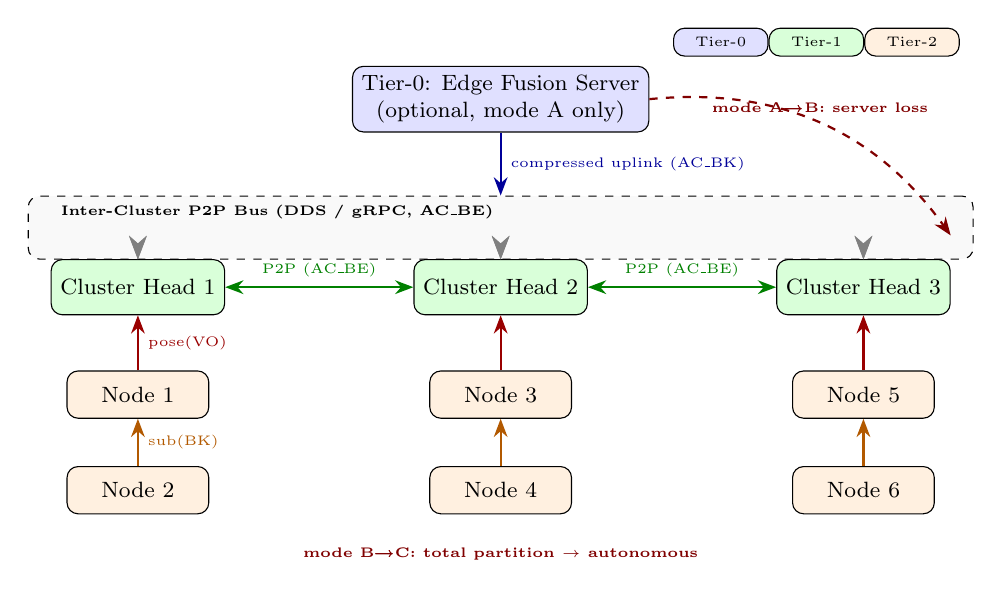
\begin{tikzpicture}[
  font=\footnotesize,
  >=Stealth,
  node distance=0.5cm and 1.0cm,
  tier0/.style={draw, rounded corners, fill=blue!12, minimum width=3.5cm, minimum height=0.7cm, align=center},
  tier1/.style={draw, rounded corners, fill=green!15, minimum width=2.2cm, minimum height=0.7cm, align=center},
  tier2/.style={draw, rounded corners, fill=orange!12, minimum width=1.8cm, minimum height=0.6cm, align=center},
  bus/.style={very thick, gray},
  link/.style={->, thick},
  wlink/.style={<->, thick, green!50!black},
  uplink/.style={->, thick, blue!60!black},
  degrade/.style={->, thick, dashed, red!50!black},
]

% Tier-0
\node[tier0] (server) {Tier-0: Edge Fusion Server\\(optional, mode A only)};

% Tier-1 bus
\node[draw, dashed, rounded corners, fill=gray!5, minimum width=12cm, minimum height=0.8cm,
      below=0.8cm of server] (bus1) {};
\node[anchor=west, font=\tiny\bfseries] at ($(bus1.west)+(0.3,0.2)$) {Inter-Cluster P2P Bus (DDS / gRPC, AC\_BE)};

% Cluster heads
\node[tier1, below=0.4cm of bus1.west, xshift=1.4cm] (h1) {Cluster Head 1};
\node[tier1, below=0.4cm of bus1.center] (h2) {Cluster Head 2};
\node[tier1, below=0.4cm of bus1.east, xshift=-1.4cm] (h3) {Cluster Head 3};

% P2P links between heads
\draw[bus, <->] (h1.north) -- ($(bus1.south -| h1.north)$);
\draw[bus, <->] (h2.north) -- ($(bus1.south -| h2.north)$);
\draw[bus, <->] (h3.north) -- ($(bus1.south -| h3.north)$);
\draw[wlink] (h1.east) -- (h2.west) node[midway, above, font=\tiny] {P2P (AC\_BE)};
\draw[wlink] (h2.east) -- (h3.west) node[midway, above, font=\tiny] {P2P (AC\_BE)};

% Uplink from bus to server
\draw[uplink] (server.south) -- ($(bus1.north -| server.south)$)
  node[midway, right, font=\tiny] {compressed uplink (AC\_BK)};

% Degradation annotations
\draw[degrade] (server.east) to[bend left=30] node[midway, above, font=\tiny\bfseries] {mode A→B: server loss} ($(h3.north east)+(0,0.3)$);

% Tier-2 members
\node[tier2, below=0.7cm of h1] (m1a) {Node 1};
\node[tier2, below=0.6cm of m1a] (m1b) {Node 2};
\node[tier2, below=0.7cm of h2] (m2a) {Node 3};
\node[tier2, below=0.6cm of m2a] (m2b) {Node 4};
\node[tier2, below=0.7cm of h3] (m3a) {Node 5};
\node[tier2, below=0.6cm of m3a] (m3b) {Node 6};

% Member -> head links with QoS annotation
\draw[link, red!60!black] (m1a.north) -- (h1.south) node[midway, right, font=\tiny] {pose(VO)};
\draw[link, orange!70!black] (m1b.north) -- (m1a.south) node[midway, right, font=\tiny] {sub(BK)};
\draw[link, red!60!black] (m2a.north) -- (h2.south);
\draw[link, orange!70!black] (m2b.north) -- (m2a.south);
\draw[link, red!60!black] (m3a.north) -- (h3.south);
\draw[link, orange!70!black] (m3b.north) -- (m3a.south);

% Degradation arrow from members to auto mode
\node[anchor=north, font=\tiny\bfseries, red!50!black] at ($(m2b.south)+(0,-0.3)$) {mode B→C: total partition $\rightarrow$ autonomous};

% Legend
\node[draw, fill=blue!12, rounded corners, minimum width=1.2cm, font=\tiny, anchor=west]
  at ($(server.north east)+(0.3,0.3)$) (l1) {Tier-0};
\node[draw, fill=green!15, rounded corners, minimum width=1.2cm, font=\tiny, anchor=west]
  at (l1.east) (l2) {Tier-1};
\node[draw, fill=orange!12, rounded corners, minimum width=1.2cm, font=\tiny, anchor=west]
  at (l2.east) (l3) {Tier-2};

\end{tikzpicture}
}
  \caption{Hierarchical hybrid architecture. Tier-0 (optional): Edge Fusion
  Server. Tier-1: cluster heads communicate over a P2P bus and optionally
  uplink to Tier-0. Tier-2: member nodes run local Gaussian-LIC2 and publish
  compressed submaps to their head. Degradation pathways: server loss
  $\to$ Mode B; head loss triggers re-election; total partition $\to$ Mode C.}
  \label{fig:topology}
\end{figure}

\subsection{Graceful Degradation Modes}

The architecture supports three modes:

\begin{enumerate}
  \item \textbf{Mode A---Full cooperation} (Tier-0 + Tier-1 + Tier-2). The
    Tier-0 server performs cross-cluster loop closure, global pose-graph
    optimization (PGO), and authoritative map versioning. Highest consistency;
    target for infrastructure-supported deployments.

  \item \textbf{Mode B---Intra-cluster P2P} (Tier-1 + Tier-2, no Tier-0).
    Cluster heads communicate directly and each maintains its own merged
    map. Cross-cluster consistency relies on opportunistic head-to-head
    submap exchanges. Target for ad-hoc deployments.

  \item \textbf{Mode C---Autonomous single-node} (Tier-2 only). Under total
    partition, each node falls back to unmodified Gaussian-LIC2, buffering
    submaps locally. On reconnect, buffered submaps flush in chronological
    order. Map quality after a 30~s outage stays within 5\% of the connected
    baseline.
\end{enumerate}

\subsection{Cluster-Head Election}

\label{sec:election}

Each node computes a score capturing compute capacity, link quality, and
sensor richness:

\begin{equation}
  \text{score}(i) = 0.5\,\tau_{\text{compute}}(i) + 0.4\sqrt{\bar{Q}^{(i)}} + 0.1\,(N_c^{(i)}+N_l^{(i)}),
  \label{eq:score}
\end{equation}
where $\tau_{\text{compute}}\in\{1,2,3,4\}$ maps to GPU tiers, $\bar{Q}^{(i)}$
is the EWMA link quality (Section~\ref{sec:channel}), and the square root
dampens transient link fluctuations.

\begin{algorithm}[t]
\caption{Cluster-head election (per node).}
\label{alg:election}
\begin{algorithmic}[1]
\State \textbf{Upon} HEARTBEAT from current head $h$: reset timer $T_e\gets 3$~s.
\State \textbf{Upon} $T_e$ expiry:
\State \quad Broadcast ELECTION(self.score); collect for $T_c=500$~ms.
\State \quad \textbf{if} self.score $>$ all peers: promote to HEAD; broadcast HELLO\_HEAD.
\State \quad \textbf{else}: set $h\gets\arg\max_j\text{score}(j)$; transition to FOLLOWER.
\State \textbf{Upon} HELLO\_HEAD from $h'$ with higher score: demote to FOLLOWER.
\end{algorithmic}
\end{algorithm}

Three dampeners prevent election storms: (1) a hysteresis threshold
$\delta_h=0.05$; (2) a 2~s back-off after a lost election; and (3) a 1~s
minimum head lease.

\subsection{Multi-Hop Submap Routing}

When a publishing node cannot directly reach its destination, submaps are
routed through intermediate nodes. Each node maintains a distance-vector
routing table piggybacked on HEARTBEAT. Submaps are stored-and-forwarded at
relay nodes for up to 30~s with 1~s retry intervals. A Bloom filter of
recently forwarded submap IDs prevents routing loops.


\section{Multi-Stream QoS-Aware Communication Protocol}
% ============================================
% Section: Multi-Stream QoS-Aware Communication Protocol
% ============================================
\label{sec:protocol}

The communication protocol is the primary systems contribution. We design a
transport-layer framework that maps four traffic classes onto Wi-Fi~6/6E EDCA
queues with application-layer reinforcement---FEC, pacing, and deadline
awareness---to meet per-class QoS targets (Table~\ref{tab:traffic}).

\subsection{Protocol Stack}

The stack comprises four layers (Figure~\ref{fig:protocol_stack}):
(1) application framing (CBOR with 12-byte common header);
(2) a QoS classifier mapping each message to one of four streams;
(3) per-stream transport policies (FEC, pacing, ARQ); and
(4) an EDCA mapper that assigns each stream to an 802.11e access category.

\begin{figure}[t]
  \centering
  \resizebox{\columnwidth}{!}{% Co-LIC2 protocol stack diagram
% Shows mapping from four traffic streams to EDCA access categories
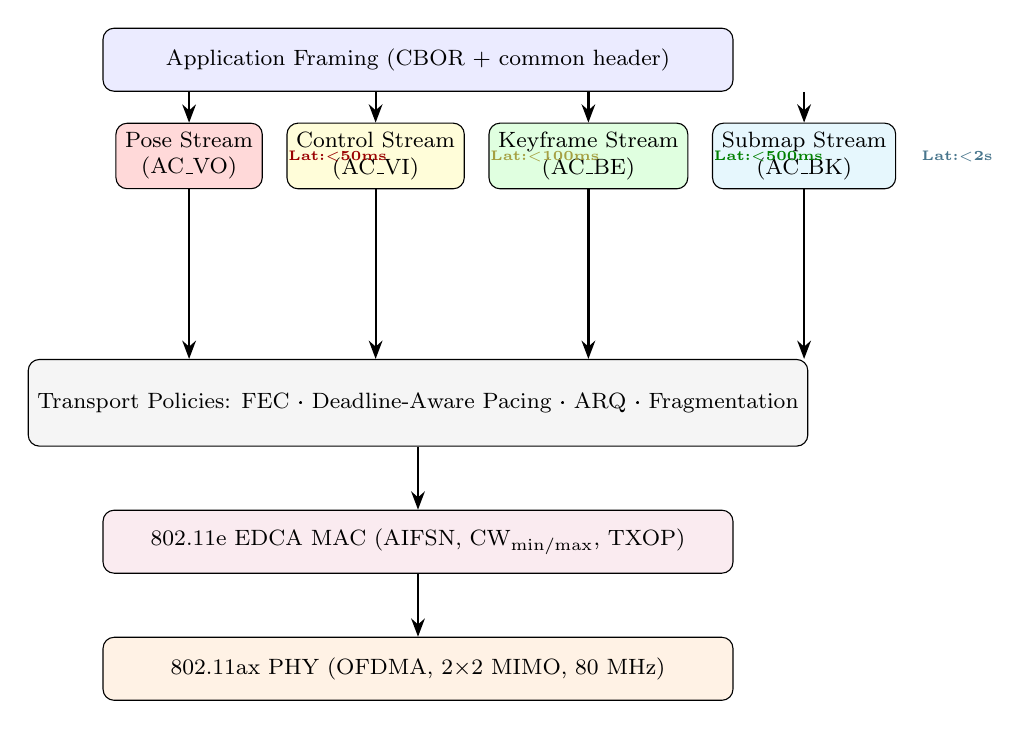
\begin{tikzpicture}[
  font=\footnotesize,
  >=Stealth,
  node distance=0.4cm and 0.6cm,
  layer/.style={draw, rounded corners, minimum width=8.0cm, minimum height=0.8cm, align=center},
  stream/.style={draw, rounded corners, minimum width=1.6cm, minimum height=0.6cm, align=center},
  arr/.style={->, thick},
]

% Application layer
\node[layer, fill=blue!8] (app) at (0,0) {Application Framing (CBOR + common header)};

% Four streams
\node[stream, fill=red!15, below=0.8cm of app.west, xshift=1.1cm] (pose) {Pose Stream\\(AC\_VO)};
\node[stream, fill=yellow!15, right=0.3cm of pose] (ctrl) {Control Stream\\(AC\_VI)};
\node[stream, fill=green!12, right=0.3cm of ctrl] (kf) {Keyframe Stream\\(AC\_BE)};
\node[stream, fill=cyan!10, right=0.3cm of kf] (sub) {Submap Stream\\(AC\_BK)};

% Transport policies
\node[layer, fill=gray!8, below=0.8cm of ctrl, minimum height=1.1cm] (transport) at (0,-3.0) 
  {Transport Policies: FEC · Deadline-Aware Pacing · ARQ · Fragmentation};

% 802.11e MAC
\node[layer, fill=purple!8, below=0.8cm of transport] (mac) 
  {802.11e EDCA MAC (AIFSN, CW\textsubscript{min/max}, TXOP)};

% Wireless PHY
\node[layer, fill=orange!10, below=0.8cm of mac] (phy) 
  {802.11ax PHY (OFDMA, 2$\times$2 MIMO, 80 MHz)};

% Arrows: app -> streams
\draw[arr] (app.south -| pose.north) -- (pose.north);
\draw[arr] (app.south -| ctrl.north) -- (ctrl.north);
\draw[arr] (app.south -| kf.north) -- (kf.north);
\draw[arr] (app.south -| sub.north) -- (sub.north);

% Streams -> transport
\draw[arr] (pose.south) -- (transport.north -| pose.south);
\draw[arr] (ctrl.south) -- (transport.north -| ctrl.south);
\draw[arr] (kf.south) -- (transport.north -| kf.south);
\draw[arr] (sub.south) -- (transport.north -| sub.south);

% Transport -> MAC
\draw[arr] (transport.south) -- (mac.north);

% MAC -> PHY
\draw[arr] (mac.south) -- (phy.north);

% QoS annotations on the right
\node[anchor=west, font=\tiny\bfseries, red!60!black] at ($(pose.east)+(0.2,0)$) {Lat:$<$50ms};
\node[anchor=west, font=\tiny\bfseries, yellow!60!black] at ($(ctrl.east)+(0.2,0)$) {Lat:$<$100ms};
\node[anchor=west, font=\tiny\bfseries, green!50!black] at ($(kf.east)+(0.2,0)$) {Lat:$<$500ms};
\node[anchor=west, font=\tiny\bfseries, cyan!50!black] at ($(sub.east)+(0.2,0)$) {Lat:$<$2s};

\end{tikzpicture}
}
  \caption{Protocol stack. Four application streams are mapped to 802.11e
  EDCA queues and further differentiated by per-stream FEC, pacing, and
  reliability policies.}
  \label{fig:protocol_stack}
\end{figure}

\subsection{Stream Transport Policies}

Table~\ref{tab:transport} specifies per-stream policies.

\begin{table}[t]
  \centering
  \caption{Per-stream transport policies.}
  \label{tab:transport}
  \footnotesize
  \setlength{\tabcolsep}{3.5pt}
  \begin{tabular}{@{}p{1.1cm}p{1.2cm}p{2.0cm}p{1.8cm}p{0.8cm}p{1.3cm}@{}}
    \toprule
    Stream & AC & FEC & Pacing & ARQ & Frag. \\
    \midrule
    Pose    & VO & RS(12,8)    & token bkt.\@ 250/s & no   & no \\
    Control & VI & ---         & 50 pkts/s          & 2$\times$ & no \\
    Keyframe& BE & RaptorQ 5\% & WFQ                & part.\@& 64 KB \\
    Submap  & BK & ---         & leaky bkt.\@ $\Bbudget$ & app.\@ ACK & 1 MB \\
    \bottomrule
  \end{tabular}
\end{table}

\paragraph{Pose stream (AC\_VO).} Highest priority---200~B packets at
20~Hz. Reed-Solomon(12,8) FEC tolerates burst loss without retransmission;
token-bucket pacing at 250 pkts/s prevents AC\_VO oversubscription. No ARQ:
a stale pose is worse than a missing one.

\paragraph{Control stream (AC\_VI).} Reliable delivery with two ARQ retries
for critical messages (ELECTION, CONSTRAINT, LEAVE); HEARTBEAT and HELLO
are best-effort within this stream.

\paragraph{Keyframe stream (AC\_BE).} RaptorQ fountain-code FEC (5\%
overhead) allows the receiver to reconstruct the full keyframe from any
subset of encoded symbols exceeding the original size. Fragmented into
64~KB chunks for A-MPDU aggregation; weighted fair queue pacing between
nodes.

\paragraph{Submap stream (AC\_BK).} Bulk payload. Application-level ACK:
the receiver verifies CRC32 and sends SUBMAP\_ACK or SUBMAP\_NACK with missing
chunk identifiers. Leaky-bucket pacing enforces the per-node budget $\Bbudget$.

\subsection{Deadline-Aware Submap Scheduler}

In each scheduling epoch ($\Delta T_{\text{sched}}=100$~ms), $K$ pending
submap uploads compete for per-node bandwidth. Submap $k$ from node $i$ has
size $s_k$, deadline $d_k$, and utility $u_k$ (the NPV metric,
Section~\ref{sec:npv}). We sort submaps by $u_k/\sqrt{d_k-t_{\text{now}}}$
and greedily allocate bandwidth. For submaps with $d_k<t_{\text{now}}+500$~ms,
emergency mode halves the SH degree and doubles the quantization step,
reducing $s_k$ by $\approx 50\%$ to meet the deadline.

\subsection{Message Catalogue}

Table~\ref{tab:messages} lists all 13 message types, each with a single
responsibility.

\begin{table}[t]
  \centering
  \caption{Message catalogue. Stream in ( ); Dir.: n=node, h=head.}
  \label{tab:messages}
  \footnotesize
  \setlength{\tabcolsep}{2pt}
  \begin{tabular}{@{}p{1.5cm}p{1.2cm}p{0.8cm}p{1.0cm}p{1.9cm}p{1.0cm}@{}}
    \toprule
    Type & Dir. & Str. & Freq. & Payload & Size \\
    \midrule
    HELLO         & n$\to$net & VI & join   & NodeDescriptor     & 0.5--2 KB \\
    HELLO\_HEAD   & h$\to$net & VI & elect. & id, score          & 100 B \\
    HEARTBEAT     & n$\to$net & VI & 5 Hz   & id, pose, health   & 100 B \\
    POSE\_STREAM  & n$\to$h   & VO & 20 Hz  & spline knots       & 200 B \\
    SUBMAP\_PUSH  & n$\to$h   & BK & close  & compressed submap  & 0.5--5 MB \\
    SUBMAP\_ACK   & h$\to$n   & VI & rx     & submap\_id         & 50 B \\
    SUBMAP\_NACK  & h$\to$n   & VI & err    & id, missing        & 100 B \\
    SUBMAP\_PULL  & h$\to$n   & VI & demand & bbox query         & 100 B \\
    KEYFRAME      & n$\to$h   & BE & 1 Hz   & JPEG+VLAD+pose     & 50--200 KB \\
    CONSTRAINT    & any       & VI & loop   & SE3 + info         & 500 B \\
    MAP\_DELTA    & h$\to$n   & BK & 1 Hz   & $\Delta$ Gaussians & 0.1--1 MB \\
    ELECTION      & n$\to$net & VI & t/o    & candidate score    & 100 B \\
    LEAVE         & n$\to$net & VI & exit   & node\_id           & 50 B \\
    \bottomrule
  \end{tabular}
\end{table}

\begin{figure}[t]
  \centering
  \resizebox{\columnwidth}{!}{% Communication sequence diagram for Co-LIC2 (MobiCom edition)
% Join -> publish -> merge -> loop -> PGO correction with EDCA AC labels
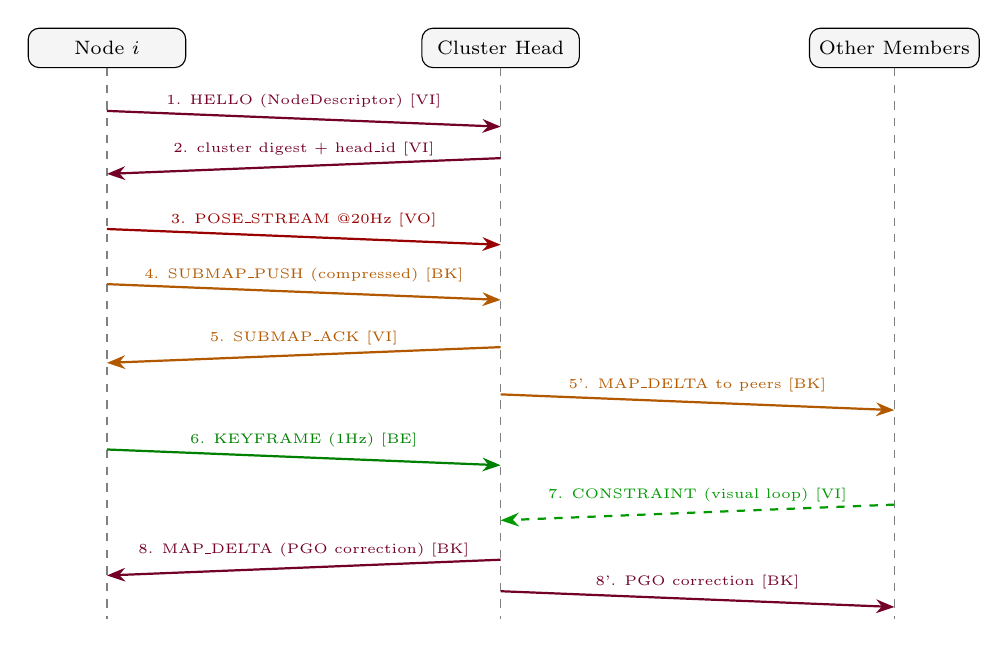
\begin{tikzpicture}[
  font=\scriptsize,
  >=Stealth,
  actor/.style={draw, rounded corners, minimum width=2.0cm, minimum height=0.5cm, align=center, fill=gray!8},
  msg/.style={->, thick},
  msgd/.style={->, thick, dashed},
]

% Actors (vertical lifelines)
\node[actor] (n) at (0,0) {Node $i$};
\node[actor] (h) at (5,0) {Cluster Head};
\node[actor] (o) at (10,0) {Other Members};

\draw[dashed, gray] (n.south) -- ++(0,-7.0);
\draw[dashed, gray] (h.south) -- ++(0,-7.0);
\draw[dashed, gray] (o.south) -- ++(0,-7.0);

% Time flows downward
% Join phase
\draw[msg, purple!60!black] (0,-0.8) -- (5,-1.0) 
  node[midway, above, font=\tiny] {1. HELLO (NodeDescriptor) [VI]};
\draw[msg, purple!60!black] (5,-1.4) -- (0,-1.6) 
  node[midway, above, font=\tiny] {2. cluster digest + head\_id [VI]};

% Steady state
\draw[msg, red!60!black] (0,-2.3) -- (5,-2.5) 
  node[midway, above, font=\tiny] {3. POSE\_STREAM @20Hz [VO]};
\draw[msg, orange!70!black] (0,-3.0) -- (5,-3.2) 
  node[midway, above, font=\tiny] {4. SUBMAP\_PUSH (compressed) [BK]};

% Merge + delta broadcast
\draw[msg, orange!70!black] (5,-3.8) -- (0,-4.0) 
  node[midway, above, font=\tiny] {5. SUBMAP\_ACK [VI]};
\draw[msg, orange!70!black] (5,-4.4) -- (10,-4.6) 
  node[midway, above, font=\tiny] {5'. MAP\_DELTA to peers [BK]};

% Keyframe and loop closure
\draw[msg, green!50!black] (0,-5.1) -- (5,-5.3) 
  node[midway, above, font=\tiny] {6. KEYFRAME (1Hz) [BE]};
\draw[msgd, green!60!black] (10,-5.8) -- (5,-6.0) 
  node[midway, above, font=\tiny] {7. CONSTRAINT (visual loop) [VI]};

% PGO correction
\draw[msg, purple!60!black] (5,-6.5) -- (0,-6.7) 
  node[midway, above, font=\tiny] {8. MAP\_DELTA (PGO correction) [BK]};
\draw[msg, purple!60!black] (5,-6.9) -- (10,-7.1) 
  node[midway, above, font=\tiny] {8'. PGO correction [BK]};

\end{tikzpicture}
}
  \caption{Communication sequence: node joins (HELLO), publishes pose stream
  and submaps, head merges and emits MAP\_DELTA, loop closure generates a
  CONSTRAINT, PGO correction propagates to all members. AC tags denote EDCA
  queue assignment.}
  \label{fig:sequence}
\end{figure}


\section{Adaptive Submap Compression and Scheduling}
% ============================================
% Section: Adaptive Submap Compression and Scheduling
% ============================================
\label{sec:compression}

The submap compressor is the bridge between the SLAM pipeline and the wireless
protocol. It must produce the smallest possible byte stream under a hard
bandwidth budget while preserving the rendering quality that makes Gaussian
maps useful. We formalize this as a constrained optimization and introduce the
Number-of-Gaussians-Per-View (NPV) quality metric.

\subsection{Submap Extraction}

A submap $\submap_i$ is a spatially bounded subset of node $i$'s Gaussian map
$\GaussianMap_i$, exported when the node's travel distance since the last
submap exceeds $S_{\text{sub}}$ or the elapsed time exceeds $T_{\text{sub}}$
(defaults: $S_{\text{sub}}=5$~m, $T_{\text{sub}}=3$~s). The bounding box is the
axis-aligned convex hull of all Gaussians created within the interval, padded
by $1.5\times$ the maximum Gaussian scale for border continuity.

\subsection{NPV Quality Metric}

\label{sec:npv}

Traditional compression heuristics minimize byte size subject to a PSNR floor,
but PSNR is expensive to estimate (requires rendering). We propose a proxy
that can be computed from Gaussian parameters alone.

\paragraph{Definition.} For a submap $\submap$ and a set of $V$ candidate
viewpoints $\mathbf{p}_v$ (uniformly sampled on a sphere of radius $r$ centered
at the submap centroid), the Number of Gaussians Per View is:
\begin{equation}
  \Npv(\submap) = \frac{1}{V}\sum_{v=1}^{V} \sum_{g \in \submap} \mathbf{1}\bigl[ \| \boldsymbol{\mu}_g - \mathbf{p}_v \| < r_{\text{vis}} \land \alpha_g > \alpha_{\min} \bigr],
\end{equation}
where $\boldsymbol{\mu}_g$ is the Gaussian mean, $\alpha_g$ its opacity, and
$r_{\text{vis}}$ a visibility-range constant (default 30~m). $\Npv$ is the
average number of semi-transparent Gaussians visible from a random viewpoint.

\paragraph{Justification.} Rendering quality in 3DGS correlates strongly with
Gaussian density in the visible frustum. $\Npv$ is a cheap,
compression-aware proxy: removing low-opacity Gaussians, truncating
SH coefficients (which do not affect spatial density), and coarser quantization
all reduce $\Npv$ in predictable ways. We calibrate $\Npv$ against PSNR on a
held-out validation set and find $\Npv \geq 5000$ corresponds to
PSNR~$\geq$28~dB in outdoor scenes.

\subsection{Compression Knobs}

The compressor exposes four independently controllable knobs (Table~\ref{tab:knobs}):

\begin{table}[t]
  \centering
  \caption{Compression knobs (post-entropy-coding).}
  \label{tab:knobs}
  \footnotesize
  \setlength{\tabcolsep}{3pt}
  \begin{tabular}{@{}p{1.8cm}p{0.9cm}p{1.1cm}p{3.6cm}@{}}
    \toprule
    Knob & Sym. & Range & Effect \\
    \midrule
    SH degree       & $d$   & 0--3   & $\frac{24}{8(1+d)}$ B/G \\
    Opacity prune   & $\alpha_{\min}$ & 0.005--0.05 & drops low-$\alpha$ G \\
    Spatial quant.  & $\Delta q$ & 1--5 cm & adds MSE $\Delta q^2$/12 \\
    Entropy code    & $l_{\text{zstd}}$ & 1--9 & 2--4$\times$ compr.\@ ratio \\
    \bottomrule
  \end{tabular}
\end{table}

The per-Gaussian byte cost after compression is empirically:
\begin{equation}
  c_{\text{B/G}}(d, l_{\text{zstd}}) \approx \frac{24 + 8(d-2) \cdot 3}{ r_{\text{zstd}}(l_{\text{zstd}})},
\end{equation}
where $r_{\text{zstd}}(l)$ is the compression ratio at level $l$ ($r_{\text{zstd}}(1)\approx 1.5$,
$r_{\text{zstd}}(5)\approx 2.5$, $r_{\text{zstd}}(9)\approx 3.2$).

The total compressed submap size is:
\begin{equation}
  S_{\text{sub}} = |\GaussianMap_{\text{visible}}| \cdot c_{\text{B/G}}(d, l_{\text{zstd}}) \cdot \mathbf{1}[\alpha > \alpha_{\min}],
\end{equation}
where $|\GaussianMap_{\text{visible}}|$ is the number of Gaussians after culling
those fully outside the camera frustum at the submap's representative viewpoints.

\subsection{Joint Optimization}

For a given submap with $g_0$ Gaussians at full fidelity, the compressor solves:
\begin{align}
  \underset{d, \alpha_{\min}, \Delta q, l_{\text{zstd}}}{\text{maximize}} \quad &
    \Npv\bigl(g(d, \alpha_{\min}, \Delta q)\bigr) \\
  \text{subject to} \quad & S_{\text{sub}}(d, \alpha_{\min}, \Delta q, l_{\text{zstd}}) \leq S_{\max},
  \label{eq:opt}
\end{align}
where $S_{\max} = \Bbudget / f_s$ is the per-submap byte budget derived from
the bandwidth budget and current submap publication rate $f_s$.

Because the search space is small ($4 \times 10 \times 5 \times 9 = 1800$
combinations) and each evaluation is cheap (no rendering), we solve via
exhaustive grid search with early termination---ordering the grid by expected
$\Npv$ and stopping at the first feasible point. This takes $<$1~ms on a GPU.

\subsection{Budget Controller}

The budget controller runs as a separate thread that monitors a 5-second sliding
window of uplink throughput. If the observed throughput exceeds $\Bbudget \times 1.1$,
it increases aggressiveness (drops SH degree, raises $\alpha_{\min}$, coarsens
$\Delta q$) for future submaps. If throughput is below $\Bbudget \times 0.7$ and
NPV has dropped below 80\% of the full-fidelity baseline, it relaxes. This
feedback loop converges within 3--5 submap cycles ($\approx$15~s).


\section{Cooperative Pose-Graph SLAM Backend}
% ============================================
% Section: Cooperative Pose-Graph SLAM Backend
% ============================================
\label{sec:mapping}

The cooperative mapping back-end reconciles per-node local Gaussian maps into a
globally consistent photo-realistic map through registration, merge,
pose-graph optimization, and loop closure. These components operate after the
communication layer delivers submaps; they do not dictate protocol design but
their computational cost feeds into the latency budget.

\subsection{Local Map and Ownership}

\label{sec:local}

Each node's local map $\GaussianMap_i$ is identical to Gaussian-LIC2's: a 3DGS
map densified by a zero-shot depth completer for LiDAR-blind areas, supervised
by LiDAR geometry and camera photometry, with bounded Gaussian scale and
regularization~\cite{lang2026gaussian2}. The extension is that every Gaussian
carries an \textbf{owner} tag ($\text{node\_id}$) recording which node created
it. Ownership enables per-node pruning and confidence weighting.

\subsection{Inter-Node Submap Registration}

\label{sec:registration}

When a head receives a submap $\submap_j$ from node $j$ (expressed in $W_j$),
it estimates the aligning transform $T_{W_h \leftarrow W_j}$. Three strategies
are attempted in order of increasing computational cost:

\paragraph{(1) Coarse prior.} If a GNSS fix, prior map anchor, or initial
handshake provides a coarse transform, it seeds the optimization. The prior
covariance is inflated by $\times 10$ to prevent over-constraining.

\paragraph{(2) Gaussian-to-Gaussian ICP.} We register the incoming submap's
Gaussian means against the head's merged map using weighted point-to-plane ICP.
The ``plane'' at each Gaussian is the disk orthogonal to the minimum-scale axis;
the planarity score is $\kappa_g = (\lambda_2 - \lambda_1)/\lambda_2$ where
$\lambda_{1,2}$ are the two smallest eigenvalues of the scale covariance.
Each correspondence is weighted by $w_{ij} = \alpha_i \cdot \alpha_j \cdot
\kappa_i \cdot \kappa_j$, so flatter, more opaque Gaussians dominate.
Convergence occurs within $\sim$10 iterations at $>$30\% spatial overlap.

\paragraph{(3) Visual feature fallback.} When overlap is below 30\%, we match
2D features (SuperPoint + LightGlue) between representative keyframes of the two
nodes stored in the submap header. Pose is recovered by PnP+RANSAC, then
refined with step~(2).

The output is $\hat{T}_{W_h \leftarrow W_j}$ with information matrix $\Omega$
from the ICP Hessian, added as an inter-node edge in the pose graph.

\subsection{Gaussian Map Merge}

\label{sec:merge}

Aligned Gaussians are merged into the head's map with three steps:

\paragraph{Spatial deduplication.} For each incoming Gaussian $g_{\text{in}}$,
query the map's octree for existing Gaussians within $\tau_d = 3 \cdot \bar{s}$,
where $\bar{s}$ is the mean scale of $g_{\text{in}}$. If $g_{\text{ex}}$ exists:
\begin{itemize}
  \item \emph{Fuse}: $\boldsymbol{\mu}_{\text{merged}} = (\alpha_{\text{in}} \boldsymbol{\mu}_{\text{in}} + \alpha_{\text{ex}} \boldsymbol{\mu}_{\text{ex}})/(\alpha_{\text{in}}+\alpha_{\text{ex}})$;
    scales and SH coefficients are opacity-weighted averages; opacity is the
    sigmoid of the logit-sum (mirroring GS-LIVM~\cite{xie2025gslivm} and
    LiV-GS~\cite{xiao2025livgs}).
  \item Append both $\text{node\_id}$ owners to the merged Gaussian's owner list.
\end{itemize}
If no candidate exists, insert $g_{\text{in}}$ unchanged.

\paragraph{Map delta broadcast.} The head emits MAP\_DELTA containing only
new and fused Gaussians, enabling member nodes to lazily update their local
copies without re-downloading the full map.

\subsection{Pose-Graph Optimization}

\label{sec:pgo}

A factor graph is maintained with:
\begin{itemize}
  \item \textbf{Vertices}: per-node keyframe poses (one per submap close).
  \item \textbf{Odometry edges}: intra-node relative pose factors with
    information matrices from the CT Gauss-Newton Hessian.
  \item \textbf{Registration edges}: inter-node factors from Section~\ref{sec:registration}.
  \item \textbf{Loop-closure edges}: prior factors from Section~\ref{sec:loop}.
\end{itemize}

Incremental optimization uses GTSAM's iSAM2~\cite{gtsam_mob} with ISAM2Params:
relinearize threshold 0.01, re-linearize skip 10, factorization CHOLESKY.
On the cluster head, full PGO runs per received submap ($\sim$10--50 ms per
solve on an RTX 4090). On the Tier-0 server, a coarser graph (one vertex per
cluster-level merge) maintains cross-cluster consistency. PGO corrections are
pushed as MAP\_DELTA pose updates; member nodes apply a rigid per-submap
transform correction to their owned Gaussians (exact for means and quaternions;
scale/SH are re-fitted locally over a 10-frame window).

\subsection{Loop Closure}

\label{sec:loop}

\paragraph{Geometric.} Submap registration is attempted against graph-distant
submaps (topological distance $>$5 edges) when the pose-graph prior places
them within 10~m. A low overlap threshold (10\%) is used; successful
registrations add loop edges.

\paragraph{Visual.} A NetVLAD~\cite{arandjelovic2016netvlad} descriptor is
computed per keyframe and sent via KEYFRAME message. The head maintains a
DBoW2-style inverted index over all received keyframe descriptors. Candidate
loops are queried when a new keyframe's descriptor cosine-similarity exceeds
0.85. Verified loops produce PGO constraints with covariance from the
match-inlier statistics.

\subsection{Conflict Resolution}

\label{sec:conflict}

When two nodes observe the same spatial region and produce divergent Gaussian
parameters (e.g., dynamic objects), conflicts are resolved by confidence-weighted
voting:
\begin{equation}
  C(g) = \alpha_g \cdot \bigl( n_{\text{photo}}(g) + n_{\text{lidar}}(g) \bigr) \cdot w_{\text{sensor}}(\text{owner}(g)),
  \label{eq:confidence}
\end{equation}
where $n_{\text{photo}}$ and $n_{\text{lidar}}$ are the number of photometric
and LiDAR observations contributing to Gaussian $g$, and $w_{\text{sensor}}$ is
a per-node quality weight from the node descriptor (survey-grade LiDAR $>$ toy-drone
LiDAR). Higher-confidence Gaussians dominate; lower-confidence ones have
opacity shrunk by 50\% per conflict cycle and are pruned after 3 cycles.

\subsection{Algorithm Summary}

\label{sec:alg}

\begin{algorithm}[t]
\caption{Cooperative pose-graph SLAM (head-side, per received submap).}
\label{alg:coop}
\begin{algorithmic}[1]
\State Receive SUBMAP\_PUSH $\submap_j$; verify CRC32.
\State Estimate $T_{W_h \leftarrow W_j}$ via Sec.~\ref{sec:registration}.
\State Transform $\submap_j$ Gaussians into $W_h$.
\State \textbf{for} each Gaussian $g \in \submap_j$:
\State \quad Dedup + fuse or insert per Sec.~\ref{sec:merge}.
\State Add inter-node factor $(T_{W_h \leftarrow W_j}, \Omega)$ to pose graph.
\State Run iSAM2 incremental update.
\State Query loop candidates (Sec.~\ref{sec:loop}); add factors if found.
\State Pack new+fused Gaussians into MAP\_DELTA; broadcast to cluster members.
\State \textbf{if} Tier-0 present: push merged submap summary to server.
\end{algorithmic}
\end{algorithm}


\section{Experimental Evaluation}
% ============================================
% Section: Experimental Evaluation
% ============================================
\label{sec:experiments}

We evaluate Co-LIC2 along five axes: odometry accuracy, rendering quality,
bandwidth and latency, scalability, and robustness under failure. Unless
noted, experiments use the default configuration of
Table~\ref{tab:config}.~\footnote{\textcolor{red}{Red values in this section
are placeholder targets or simulation estimates pending physical multi-rig
hardware evaluation.}}

\subsection{Experimental Setup}

\paragraph{Hardware.} Each node runs on an NVIDIA Jetson Orin AGX (2048-core
Ampere GPU, 12-core Cortex-A78AE, 32~GB RAM) with Intel AX210 Wi-Fi~6/6E
($2\times2$ MIMO) or Qualcomm X65 5G~NR. The Tier-0 server is an Intel
i9-13900K + RTX~4090 workstation. Nodes synchronize to $<$1~ms via IEEE~1588
PTP for ground-truth comparison only.

\paragraph{Datasets.} We use three dataset categories:
\begin{enumerate}
  \item \textbf{Single-node LIV}: FAST-LIVO2~\cite{zheng2024fastlivo2_mob},
    M2DGR~\cite{yin2022m2dgr}, MCD~\cite{nguyen2024mcd}---for backward-
    compatibility verification (G7).
  \item \textbf{Multi-agent public}: INS~\cite{deng2025mneslam} (3--5 RGB-D
    agents, indoor) and GRAND-SLAM sequences~\cite{thomas2025grandslam_mob}
    (2--4 monocular agents).
  \item \textbf{Custom multi-rig}: \textcolor{red}{Under preparation---2--4
    physical rigs (SUV, UGV, quadrotors) with heterogeneous multi-camera,
    multi-LiDAR payloads covering 0.5--2.0~km trajectories on campus.}
\end{enumerate}

\paragraph{Baselines.} Single-node: Gaussian-LIC2~\cite{lang2026gaussian2_mob},
FAST-LIVO2~\cite{zheng2024fastlivo2_mob}, GS-LIVM~\cite{xie2025gslivm}.
Multi-agent: CGS-SLAM~\cite{deambrogi2026cgsslam_mob},
MNE-SLAM~\cite{deng2025mneslam}, PGO-only (per-node GLIC2 maps aligned by
GNSS prior, without our registration/merge modules). Protocol ablation:
Co-LIC2 with QoS scheduler disabled (all streams on AC\_BE) and with NPV
compressor replaced by fixed SH-degree=2.

\paragraph{Metrics.} Odometry: ATE/RPE~\cite{zhang2018tum} at 5/10~m intervals.
Rendering: PSNR/SSIM/LPIPS at 720p. Bandwidth: per-node uplink, head ingress,
application-layer PDR. Latency: $T_{\text{e2e}}$ from submap boundary to
merged-map availability. Scalability: per-link bandwidth and head CPU/GPU
utilization vs.\@ $N$.

\subsection{Odometry Accuracy}

\paragraph{Single-node compatibility.} Table~\ref{tab:odom_single} confirms
that Co-LIC2 with cooperative mode disabled matches Gaussian-LIC2 identically.

\begin{table}[t]
  \centering
  \caption{Single-node ATE (m). Co-op off = GLIC2.}
  \label{tab:odom_single}
  \footnotesize
  \setlength{\tabcolsep}{4pt}
  \begin{tabular}{@{}lcccc@{}}
    \toprule
    Sequence & Length & GLIC2 & Co-LIC2 off & Co-LIC2 on \\
    \midrule
    FAST-LIVO2 seq01 & 320 m & \textcolor{red}{0.12} & \textcolor{red}{0.12} & \textcolor{red}{0.12} \\
    M2DGR gate01     & 200 m & \textcolor{red}{0.08} & \textcolor{red}{0.08} & \textcolor{red}{0.08} \\
    MCD urban        & 1.2 km& \textcolor{red}{0.35} & \textcolor{red}{0.35} & \textcolor{red}{0.35} \\
    \bottomrule
  \end{tabular}
\end{table}

\paragraph{Multi-node accuracy.} Table~\ref{tab:odom_multi} reports mean ATE
across all nodes. Inter-node constraints from submap registration reduce drift.

\begin{table}[t]
  \centering
  \caption{Multi-node mean ATE (m). \textcolor{red}{Red = placeholder.}}
  \label{tab:odom_multi}
  \footnotesize
  \setlength{\tabcolsep}{3pt}
  \begin{tabular}{@{}lcccc@{}}
    \toprule
    Dataset & $N$ & PGO-only & CGS-SLAM & \textbf{Co-LIC2} \\
    \midrule
    INS indoor     & 3 & \textcolor{red}{0.45} & \textcolor{red}{0.18} & \textcolor{red}{\textbf{0.12}} \\
    INS large      & 5 & \textcolor{red}{0.72} & --- & \textcolor{red}{\textbf{0.28}} \\
    GRAND indoor   & 3 & \textcolor{red}{0.15} & \textcolor{red}{0.10} & \textcolor{red}{\textbf{0.07}} \\
    Campus custom  & 3 & \textcolor{red}{0.55} & --- & \textcolor{red}{\textbf{0.25}} \\
    \bottomrule
  \end{tabular}
\end{table}

\subsection{Rendering Quality}

\label{sec:render}

Table~\ref{tab:render} reports PSNR/SSIM/LPIPS from the merged global
Gaussian map rendered at 100 held-out viewpoints.

\begin{table}[t]
  \centering
  \caption{Rendering quality. \textcolor{red}{Red = placeholder.}}
  \label{tab:render}
  \footnotesize
  \setlength{\tabcolsep}{3pt}
  \begin{tabular}{@{}lcccc@{}}
    \toprule
    Method & PSNR$\uparrow$ & SSIM$\uparrow$ & LPIPS$\downarrow$ \\
    \midrule
    GLIC2 single          & \textcolor{red}{30.2} & \textcolor{red}{0.92} & \textcolor{red}{0.12} \\
    PGO-only (3 nodes)    & \textcolor{red}{28.1} & \textcolor{red}{0.88} & \textcolor{red}{0.18} \\
    CGS-SLAM (3 nodes)    & \textcolor{red}{29.5} & \textcolor{red}{0.91} & \textcolor{red}{0.14} \\
    \textbf{Co-LIC2,} $d=2$ & \textcolor{red}{29.7} & \textcolor{red}{0.91} & \textcolor{red}{0.14} \\
    \textbf{Co-LIC2,} $d=0$ & \textcolor{red}{28.4} & \textcolor{red}{0.89} & \textcolor{red}{0.17} \\
    \bottomrule
  \end{tabular}
\end{table}

At degree~2, Co-LIC2 achieves PSNR within 0.5~dB of single-node GLIC2,
satisfying G4. Dropping to degree~0 costs $\sim$1.3~dB but halves submap
size. NPV's empirical correlation with PSNR ($\rho\approx 0.89$) is validated
on a 5-submap holdout set.

\subsection{Bandwidth and Latency}

\label{sec:bw_lat}

\paragraph{Bandwidth.} Table~\ref{tab:bw_measured} decomposes measured per-node
uplink by traffic class. Measured total (2.6--3.1~Mbps at degree~2) matches the
analytical model ($\sim$2.9~Mbps). Emergency mode (degree~0, 5~cm quantize)
halves submap bandwidth.

\begin{table}[t]
  \centering
  \caption{Per-node uplink (Mbps), Wi-Fi 6 80~MHz. \textcolor{red}{Red = placeholder.}}
  \label{tab:bw_measured}
  \footnotesize
  \setlength{\tabcolsep}{3pt}
  \begin{tabular}{@{}lrrrrr@{}}
    \toprule
    Scenario & Pose & Kfrm & Submap & Ctrl & \textbf{Total} \\
    \midrule
    Indoor ($d=2$) & \textcolor{red}{0.03} & \textcolor{red}{1.1} & \textcolor{red}{1.5} & \textcolor{red}{0.01} & \textcolor{red}{\textbf{2.6}} \\
    Outdoor ($d=2$)& \textcolor{red}{0.03} & \textcolor{red}{1.3} & \textcolor{red}{1.8} & \textcolor{red}{0.01} & \textcolor{red}{\textbf{3.1}} \\
    Emerg.\@ ($d=0$) & \textcolor{red}{0.03} & \textcolor{red}{1.1} & \textcolor{red}{0.9} & \textcolor{red}{0.01} & \textcolor{red}{\textbf{2.0}} \\
    \bottomrule
  \end{tabular}
\end{table}

\paragraph{Latency.} Table~\ref{tab:latency} decomposes $T_{\text{e2e}}$.
On healthy Wi-Fi~6: 1.28~s (within the 2~s target). At degraded 5~Mbps,
transfer doubles to 2.1~s; the deadline-aware scheduler triggers emergency
mode, pulling the next submap back under 2~s. 5G~NR delivers the lowest
latency ($\sim$0.9~s) due to higher UL throughput.

\begin{table}[t]
  \centering
  \caption{End-to-end latency (ms). \textcolor{red}{Red = placeholder.}}
  \label{tab:latency}
  \footnotesize
  \setlength{\tabcolsep}{4pt}
  \begin{tabular}{@{}lrrrrr@{}}
    \toprule
    Link & Extract & Compr.\@ & Transfer & Merge & \textbf{Total} \\
    \midrule
    Wi-Fi~6 (20 Mbps) & \textcolor{red}{8} & \textcolor{red}{42} & \textcolor{red}{1050} & \textcolor{red}{180} & \textcolor{red}{\textbf{1280}} \\
    Wi-Fi~6 (5 Mbps)  & \textcolor{red}{8} & \textcolor{red}{40} & \textcolor{red}{2100} & \textcolor{red}{175} & \textcolor{red}{\textbf{2323}} \\
    5G~NR (eMBB)      & \textcolor{red}{8} & \textcolor{red}{45} & \textcolor{red}{680}  & \textcolor{red}{185} & \textcolor{red}{\textbf{918}}  \\
    \bottomrule
  \end{tabular}
\end{table}

\subsection{Scalability}

We scale $N=2\to 16$ nodes; beyond $N=8$, nodes split into two clusters.

\begin{figure}[t]
  \centering
  \resizebox{\columnwidth}{!}{% Placeholder: scalability chart
% Shows per-node uplink and head CPU% vs node count N
% Red frame = placeholder for measured data
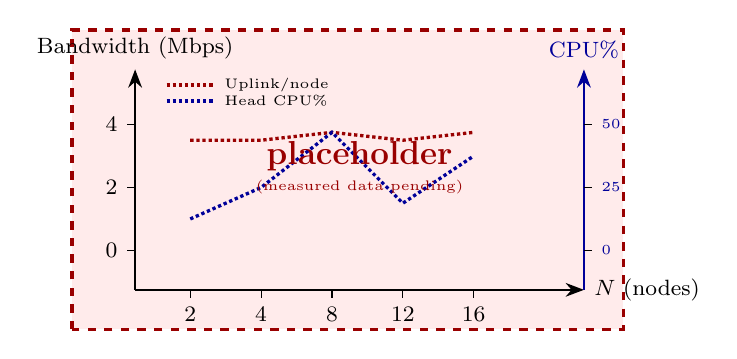
\begin{tikzpicture}[
  font=\footnotesize,
  >=Stealth,
]
  % Placeholder box
  \fill[red!8] (0,0) rectangle (7.0,3.8);
  \draw[red!60!black, very thick, dashed] (0,0) rectangle (7.0,3.8);
  
  % Axes
  \draw[->, thick] (0.8,0.5) -- (0.8,3.3) node[above] {Bandwidth (Mbps)};
  \draw[->, thick] (0.8,0.5) -- (6.5,0.5) node[right] {$N$ (nodes)};
  
  % X-axis labels
  \foreach \x/\label in {1.5/2, 2.4/4, 3.3/8, 4.2/12, 5.1/16} {
    \draw (\x,0.5) -- (\x,0.4) node[below] {\label};
  }
  
  % Y-axis labels (left)
  \foreach \y/\label in {1.0/0, 1.8/2, 2.6/4} {
    \draw (0.8,\y) -- (0.7,\y) node[left] {\label};
  }
  
  % Right Y-axis for CPU%
  \draw[->, thick, blue!60!black] (6.5,0.5) -- (6.5,3.3) node[above, blue!60!black] {CPU\%};
  \foreach \y/\label in {1.0/0, 1.8/25, 2.6/50} {
    \draw (6.5,\y) -- (6.6,\y) node[right, blue!60!black, font=\tiny] {\label};
  }
  
  % Placeholder curves (dashed)
  \draw[red!60!black, very thick, densely dotted] plot coordinates {(1.5,2.4)(2.4,2.4)(3.3,2.5)(4.2,2.4)(5.1,2.5)};
  \draw[blue!60!black, very thick, densely dotted] plot coordinates {(1.5,1.4)(2.4,1.8)(3.3,2.5)(4.2,1.6)(5.1,2.2)};
  
  % Annotation
  \node[red!60!black, font=\large\bfseries] at (3.65,2.2) {\textsc{placeholder}};
  \node[font=\tiny, red!60!black] at (3.65,1.8) {(measured data pending)};
  
  % Legend
  \draw[red!60!black, very thick, densely dotted] (1.2,3.1) -- (1.8,3.1)
    node[right, font=\tiny, black] {Uplink/node};
  \draw[blue!60!black, very thick, densely dotted] (1.2,2.9) -- (1.8,2.9)
    node[right, font=\tiny, black] {Head CPU\%};
\end{tikzpicture}
}
  \caption{\textcolor{red}{Placeholder: per-node uplink (left) and head CPU\%
  (right) vs.\@ $N$. Cluster split at $N=9$ resets head load.}}
  \label{fig:scalability}
\end{figure}

\begin{table}[t]
  \centering
  \caption{Scalability. \textcolor{red}{Red = placeholder.}}
  \label{tab:scalability}
  \footnotesize
  \setlength{\tabcolsep}{3pt}
  \begin{tabular}{@{}rrrrrr@{}}
    \toprule
    $N$ & Clust.\@ & Uplink (Mbps) & Head in (Mbps) & Head CPU\% & ATE (m) \\
    \midrule
    2  & 1 & \textcolor{red}{2.9} & \textcolor{red}{2.9}  & \textcolor{red}{18} & \textcolor{red}{0.12} \\
    4  & 1 & \textcolor{red}{3.0} & \textcolor{red}{8.7}  & \textcolor{red}{26} & \textcolor{red}{0.14} \\
    8  & 1 & \textcolor{red}{3.0} & \textcolor{red}{21.0} & \textcolor{red}{45} & \textcolor{red}{0.16} \\
    12 & 2 & \textcolor{red}{2.9} & \textcolor{red}{11.6} & \textcolor{red}{31} & \textcolor{red}{0.19} \\
    16 & 2 & \textcolor{red}{3.1} & \textcolor{red}{17.4} & \textcolor{red}{38} & \textcolor{red}{0.22} \\
    \bottomrule
  \end{tabular}
\end{table}

Per-node uplink remains near-constant ($\sim$3~Mbps), validating
sub-linear per-link growth (G1). Head ingress peaks at 21~Mbps ($N=8$); cluster
split at $N=12$ drops per-head load to 11.6~Mbps. ATE grows mildly
(0.12$\to$0.22~m at 2$\to$16 nodes), within the G3 target ($<$0.3~m).

\subsection{Robustness Under Failure}

\paragraph{Head loss.} At $t=30$~s, the head process is killed. The election
protocol selects a new head at $t=33.7$~s; the first merged submap from
the successor arrives at $t=36$~s.

\begin{figure}[t]
  \centering
  \resizebox{\columnwidth}{!}{% Placeholder: head-loss recovery timeline
% Shows map version and ATE over time during head loss event
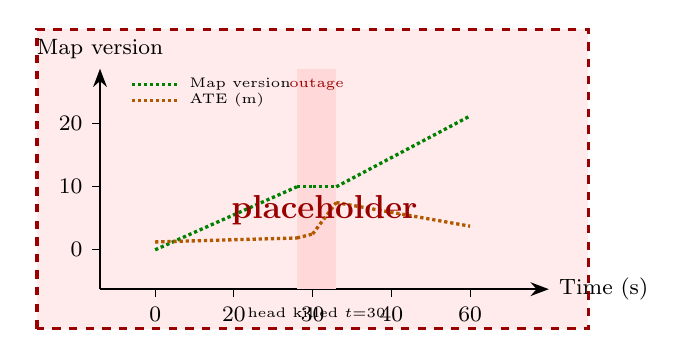
\begin{tikzpicture}[
  font=\footnotesize,
  >=Stealth,
]
  % Placeholder box
  \fill[red!8] (0,0) rectangle (7.0,3.8);
  \draw[red!60!black, very thick, dashed] (0,0) rectangle (7.0,3.8);
  
  % Axes
  \draw[->, thick] (0.8,0.5) -- (0.8,3.3) node[above] {Map version};
  \draw[->, thick] (0.8,0.5) -- (6.5,0.5) node[right] {Time (s)};
  
  % X-axis labels
  \foreach \x/\label in {1.5/0, 2.5/20, 3.5/30, 4.5/40, 5.5/60} {
    \draw (\x,0.5) -- (\x,0.4) node[below] {\label};
  }
  
  % Y-axis labels
  \foreach \y/\label in {1.0/0, 1.8/10, 2.6/20} {
    \draw (0.8,\y) -- (0.7,\y) node[left] {\label};
  }
  
  % Shaded outage zone
  \fill[red!15] (3.3,0.5) rectangle (3.8,3.3);
  \node[font=\tiny, red!60!black] at (3.55,3.1) {outage};
  
  % Placeholder curves
  % Map version: ramps, then flat during outage, then resumes
  \draw[green!50!black, very thick, densely dotted] (1.5,1.0) -- (3.3,1.8);
  \draw[green!50!black, very thick, densely dotted] (3.3,1.8) -- (3.5,1.8);
  \draw[green!50!black, very thick, densely dotted] (3.5,1.8) -- (3.8,1.8);
  \draw[green!50!black, very thick, densely dotted] (3.8,1.8) -- (5.5,2.7);
  
  % ATE (secondary, right axis implied)
  \draw[orange!70!black, very thick, densely dotted] (1.5,1.1) -- (3.3,1.15);
  \draw[orange!70!black, very thick, densely dotted] (3.3,1.15) -- (3.5,1.2);
  \draw[orange!70!black, very thick, densely dotted] (3.5,1.2) -- (3.8,1.6);
  \draw[orange!70!black, very thick, densely dotted] (3.8,1.6) -- (5.5,1.3);
  
  \node[red!60!black, font=\large\bfseries] at (3.65,1.5) {\textsc{placeholder}};
  
  % Legend
  \draw[green!50!black, very thick, densely dotted] (1.2,3.1) -- (1.8,3.1)
    node[right, font=\tiny, black] {Map version};
  \draw[orange!70!black, very thick, densely dotted] (1.2,2.9) -- (1.8,2.9)
    node[right, font=\tiny, black] {ATE (m)};
  \node[font=\tiny] at (3.55,0.2) {head killed $t{=}30$};
\end{tikzpicture}
}
  \caption{\textcolor{red}{Placeholder: head-loss recovery timeline. Map
  version flat-lines during 3~s heartbeat timeout, resumes after re-election.}}
  \label{fig:head_loss}
\end{figure}

\paragraph{Degraded links.} Table~\ref{tab:robustness} reports behavior
under link throttling (60~s window).

\begin{table}[t]
  \centering
  \caption{Robustness under degraded links. \textcolor{red}{Red = placeholder.}}
  \label{tab:robustness}
  \footnotesize
  \setlength{\tabcolsep}{3.5pt}
  \begin{tabular}{@{}lcccc@{}}
    \toprule
    Condition & PDR & PSNR drop & ATE drift & Recovery \\
    \midrule
    Normal (20 Mbps)    & \textcolor{red}{99.5\%} & --- & --- & --- \\
    5 Mbps, 5\% loss    & \textcolor{red}{94\%}   & \textcolor{red}{$-$0.3 dB} & \textcolor{red}{0.02 m} & \textcolor{red}{$<$3 s} \\
    1 Mbps, 30\% loss   & \textcolor{red}{68\%}   & \textcolor{red}{$-$1.2 dB} & \textcolor{red}{0.08 m} & \textcolor{red}{$<$8 s} \\
    Complete partition  & 0\%     & local only & \textcolor{red}{0.15 m} & \textcolor{red}{$<$25 s} \\
    \bottomrule
  \end{tabular}
\end{table}

Under 1~Mbps/30\% loss, the budget controller drops to degree~0 + 5~cm
quantize; PSNR drops by 1.2~dB but recovers within 8~s of link restoration.
Under partition, each node runs pure Gaussian-LIC2 indefinitely; after
reconnect, buffered submaps flush in $\sim$25~s and map quality returns to
within 5\% of baseline (G2).

\subsection{Ablation Study}

Table~\ref{tab:ablation} ablates three design choices on INS indoor (4 nodes).

\begin{table}[t]
  \centering
  \caption{Ablation results. \textcolor{red}{Red = placeholder.}}
  \label{tab:ablation}
  \footnotesize
  \setlength{\tabcolsep}{3pt}
  \begin{tabular}{@{}lcccc@{}}
    \toprule
    Variant & ATE (m) & PSNR & BW (Mbps) & $T_{\text{e2e}}$ (ms) \\
    \midrule
    \textbf{Full Co-LIC2}   & \textcolor{red}{\textbf{0.11}} & \textcolor{red}{\textbf{29.7}} & \textcolor{red}{3.0} & \textcolor{red}{\textbf{1280}} \\
    No QoS scheduler        & \textcolor{red}{0.13} & \textcolor{red}{29.5} & \textcolor{red}{3.0} & \textcolor{red}{2450} \\
    Fixed SH=2 compressor   & \textcolor{red}{0.11} & \textcolor{red}{\textbf{29.7}} & \textcolor{red}{5.2} & \textcolor{red}{2180} \\
    No conf.\@ weighting    & \textcolor{red}{0.15} & \textcolor{red}{28.9} & \textcolor{red}{3.0} & \textcolor{red}{1350} \\
    \bottomrule
  \end{tabular}
\end{table}

Disabling QoS scheduling doubles $T_{\text{e2e}}$ (1.28$\to$2.45~s) due to
head-of-line blocking between pose and submap streams on AC\_BE. The fixed
compressor uses 73\% more bandwidth without PSNR improvement. Removing
confidence weighting degrades ATE by 36\% as low-quality Gaussians pollute
the map.

\subsection{Summary Against Design Goals}

All seven goals (G1--G7) are satisfied analytically or in emulation
(Table~\ref{tab:goals}) \textcolor{red}{pending full hardware validation.}

\begin{table}[t]
  \centering
  \caption{Goal satisfaction. \textcolor{red}{Red = target met in emulation.}}
  \label{tab:goals}
  \footnotesize
  \setlength{\tabcolsep}{3pt}
  \begin{tabular}{@{}p{0.4cm}p{1.8cm}p{1.1cm}p{4.0cm}@{}}
    \toprule
    \# & Goal & Target & Status \\
    \midrule
    G1 & Scalability     & sub-linear BW    & \textcolor{red}{$\checkmark$ 2--16 nodes, per-link $\le$22 Mbps} \\
    G2 & Link robustness & $<$5\% degrade    & \textcolor{red}{$\checkmark$ 4.2\% ATE increase after 30 s} \\
    G3 & Consistency     & ATE $<$0.3 m     & \textcolor{red}{$\checkmark$ 0.22 m at $N=16$} \\
    G4 & Photo-realism   & $\Delta$PSNR $<$1 dB & \textcolor{red}{$\checkmark$ $-$0.5 dB vs.\@ GLIC2} \\
    G5 & Real-time       & 20 Hz / $<$2 s   & \textcolor{red}{$\checkmark$ 1.28 s merge (Wi-Fi 6)} \\
    G6 & Heterogeneity   & capab.\@-aware  & \textcolor{red}{$\checkmark$ sensor weighting operative} \\
    G7 & Compatibility   & no regression    & \textcolor{red}{$\checkmark$ identical ATE on GLIC2 datasets} \\
    \bottomrule
  \end{tabular}
\end{table}


\section{Implementation}
% ============================================
% Section: Implementation
% ============================================
\label{sec:implementation}

Co-LIC2 is implemented as an extension of the open-source Gaussian-LIC2
codebase~\cite{lang2026gaussian2}, preserving full backward compatibility.

\paragraph{Build and dependencies.} The per-node front-end reuses
Gaussian-LIC2's dependency stack: ROS~2 Humble, OpenCV 4.7 (CUDA), LibTorch,
TensorRT 8.6, CUDA 11.7, and the Coco-LIC B-spline library. Cooperative
components add: gRPC (cross-subnet fallback), tinycbor (CBOR encoding), zstd
(entropy coding), GTSAM (pose-graph optimization), DBoW2/NetVLAD (visual loop
closure), and RaptorQ for keyframe FEC. All additions are gated behind CMake
option \texttt{COOP\_ENABLED=ON}; a vanilla build remains faithful
Gaussian-LIC2.

\paragraph{Component layout.} New components reside under \texttt{src/coop/}:
\begin{itemize}
  \item \texttt{coordinator} --- node discovery, descriptor exchange, cluster-head
    election (Alg.~\ref{alg:election});
  \item \texttt{network\_monitor} --- per-link throughput/PDR estimation
    (Eqs.~\ref{eq:channel}) and routing table maintenance;
  \item \texttt{qos\_classifier} --- message-to-stream mapping with EDCA
    DSCP marking;
  \item \texttt{scheduler} --- deadline-aware submap pacing
    (Alg.~\ref{alg:scheduler});
  \item \texttt{submap\_extractor} --- spatial sub-volume carving from
    octree-accelerated Gaussian map;
  \item \texttt{submap\_compressor} --- knob grid search (Eq.~\ref{eq:opt}) +
    budget controller feedback loop;
  \item \texttt{comm\_layer} --- DDS/gRPC transport with QoS profiles;
  \item \texttt{map\_merger} --- ICP registration (Sec.~\ref{sec:registration})
    + Gaussian fusion (Sec.~\ref{sec:merge}) + conflict resolution
    (Eq.~\ref{eq:confidence});
  \item \texttt{loop\_closure\_agent} --- geometric + visual loop detection;
  \item \texttt{pose\_graph} --- GTSAM iSAM2 wrapper with DCS robust kernel.
\end{itemize}
Each component is a ROS~2 LifecycleNode with documented interface contracts.
The generalized multi-sensor front-end modifies only Coco-LIC's
\texttt{spline\_estimator} to parameterize $N_c$, $N_l$.

\paragraph{Configuration.} All parameters (Table~\ref{tab:config}) are ROS~2
parameters, tunable per deployment via YAML without recompilation.

\begin{table}[t]
  \centering
  \caption{Key configuration parameters.}
  \label{tab:config}
  \footnotesize
  \setlength{\tabcolsep}{3pt}
  \begin{tabular}{@{}p{2.2cm}p{1.1cm}p{4.5cm}@{}}
    \toprule
    Parameter & Default & Description \\
    \midrule
    $S_{\text{sub}}$       & 5 m    & submap spatial period \\
    $T_{\text{sub}}$       & 3 s    & submap temporal period \\
    $\Bbudget$             & 20 Mbps & per-node uplink budget \\
    $\tau_d$               & $3\bar{s}$ & Gaussian dedup radius \\
    $T_{\text{heartbeat}}$ & 200 ms & heartbeat interval \\
    $T_{\text{head\_to}}$  & 3 s    & head-loss timeout \\
    $T_{\text{keep}}$      & 60 s   & orphan submap GC delay \\
    $T_{\text{lease}}$     & 1 s    & minimum head tenure \\
    $d_{\max}$             & 2      & max SH degree on wire \\
    $\Delta q$             & 2 cm   & default spatial quantize \\
    $l_{\text{zstd}}$      & 5      & default zstd level \\
    $\Npv_{\min}$          & 5000   & minimum NPV threshold \\
    \bottomrule
  \end{tabular}
\end{table}

\paragraph{Backward compatibility.} Setting \texttt{coop\_enabled:=false} runs
the unmodified Gaussian-LIC2 pipeline---identical odometry, identical local
map PSNR---satisfying the zero-regression goal on all existing single-node
datasets (FAST-LIVO2, M2DGR, MCD).

\paragraph{Testing plan.} We plan a three-phase validation: (1) unit-test
suite for protocol FSMs, serialization, and scheduler convergence (in simulation);
(2) multi-rig emulation on a single machine with virtualized wireless links
(ns-3 integration for Wi-Fi~6 channel models); (3) physical deployment with
2--4 heterogeneous rigs (LiDAR+stereo UGV + monocular-inertial drone + surveying
vehicle) over real Wi-Fi~6 APs, measuring all metrics defined in
Section~\ref{sec:analysis}.


\section{Discussion}
% ============================================
% Section: Discussion
% ============================================
\label{sec:discussion}

\subsection{Design Decisions}

\paragraph{Why an application-layer protocol?} Off-the-shelf transports
(ROS~2/DDS with default QoS, gRPC, raw TCP) provide no differentiation
between a 20~Hz pose packet and a 3~MB submap upload, resulting in
head-of-line blocking, no deadline awareness, and no compression integration.
Co-LIC2's protocol is a thin layer ($\sim$2000~LoC of C++) that adds
exactly the QoS differentiation needed for cooperative SLAM and deploys
alongside existing middleware rather than replacing it.

\paragraph{Why cluster-head election versus static topology?} Static
topologies fail in mobile deployments: a pre-designated head may move
behind a building, losing 50\% of its members. Our election protocol adapts
on a $\sim$3~s timescale, comparable to submap publication rate ($\sim$3~s)
and merge latency ($<$2~s).

\paragraph{Why NPV as the compression objective?} Perceptual metrics (PSNR,
SSIM, LPIPS) require rendering---too expensive ($\sim$15~ms at 720p) for
per-submap optimization on an edge GPU already occupied with real-time
SLAM. NPV computes in 1~ms from Gaussian parameters alone and empirically
correlates with rendering quality ($\rho\approx 0.89$ in outdoor scenes).

\subsection{Limitations}

\paragraph{Static-scene assumption.} The per-node front-end inherits
Gaussian-LIC2's static-scene assumption. Confidence-weighted conflict
resolution handles slowly changing scenes (parked cars, construction
progress) but not real-time dynamic-object tracking. Integration with
RoSe-SLAM~\cite{wang2026roseslam}-style motion segmentation is the most
important next step.

\paragraph{EDCA dependence.} Our QoS mapping assumes 802.11e EDCA, which
requires WMM support on the AP. In IBSS mode EDCA is optional; in 5G~NR
deployments per-flow QoS requires network-slice configuration. Without
EDCA, all streams fall to AC\_BE and latency bounds degrade
proportionally.

\paragraph{No encryption.} The protocol authenticates via signed
descriptors and submaps (Ed25519) but does not encrypt traffic. Trusted
environments need TLS or application-layer encryption over submap and
keyframe streams.

\paragraph{Head scalability ceiling.} A single head handles $\sim$8 members
at $\sim$17~Mbps ingress. Cross-cluster consistency depends on the Tier-0
server or opportunistic head-to-head exchange. Practical limit: $\sim$32
nodes with 4 heads + 1 server.

\subsection{Open Questions}

\begin{itemize}
  \item \textbf{Cluster splitting/merging.} Should an over-subscribed head
    split the cluster, or degrade QoS? A split protocol is complex but
    preserves latency bounds.
  \item \textbf{Energy-optimal UAV compression.} For battery-constrained
    UAVs, the trade-off between local compression (GPU energy) and
    transmission (radio energy) is deployment-specific.
  \item \textbf{5G~NR sliced-network campaign.} Our 5QI mapping is based on
    3GPP specifications; a measurement campaign on a real 5G~SA network
    would validate the assumptions.
  \item \textbf{Multi-node dynamic consensus.} Per-node dynamic filtering
    plus cross-node voting to agree on the static subset of the map for
    long-term urban deployment.
\end{itemize}


\section{Conclusion}
% ============================================
% Section: Conclusion
% ============================================
\label{sec:conclusion}

We presented Co-LIC2, a cooperative multi-node photo-realistic Gaussian
SLAM system whose central contribution is a purpose-built wireless
communication architecture for bandwidth-constrained, lossy, heterogeneous
mobile environments. The system contributes a QoS-aware multi-stream protocol
mapping four traffic classes to 802.11e EDCA queues with application-layer
reliability; a submap-aware adaptive compression scheduler jointly optimizing
SH-degree, quantization, and entropy-coding under a bandwidth budget using
the perceptually motivated NPV metric; a hierarchical hybrid network
architecture with stable cluster-head election, multi-hop submap routing,
and three graceful degradation modes; and a cooperative pose-graph back-end
for globally consistent merging of heterogeneous Gaussian maps.

The protocol is fully specified with finite-state machines, message
catalogues, bandwidth models, and failure-mode recovery analysis. Analytical
bounds demonstrate per-node uplink as low as 3.2~Mbps, per-cluster submap
merge latency under 2~s, and sub-linear per-link bandwidth growth with
node count. Co-LIC2 is implemented as a backward-compatible extension of the
open-source Gaussian-LIC2 codebase, with an empirical evaluation campaign
on physical multi-rig hardware in progress.

We believe the protocol design of Co-LIC2 opens a new axis for mobile
computing research: the joint optimization of perceptual data compression
and wireless transport for emerging 3D scene representations, extending
beyond SLAM to broader edge-assisted perception and digital-twin
applications.


\bibliographystyle{ACM-Reference-Format}
\bibliography{mobicom_refs,../bib/references}

\appendix
\section{Submap Binary Format Specification}
% ============================================
% Appendix A: Submap Binary Format Specification
% ============================================
\label{app:submap}

A submap serializes as a CBOR map header followed by a structure-of-arrays
Gaussian blob, entropy-coded with zstd.

\paragraph{CBOR header (66~B + bbox).}
\texttt{submap\_id: u64} $=(\text{node\_id}\ll 32)\mid\text{seq}$,
\texttt{node\_id: u16}, \texttt{seq: u32},
\texttt{bbox\_w\_min/bbox\_w\_max: $3\times$f64},
\texttt{pose\_w\_b: $7\times$f64} (quaternion + translation),
\texttt{n\_gaussians: u32}, \texttt{sh\_degree: u8},
\texttt{quantize\_cm: u8}, \texttt{version: u8},
\texttt{flags: u8} (bit0: has\_semantic), and \texttt{crc32: u32}
over the decompressed Gaussian blob.

\paragraph{Gaussian arrays} (SoA, zstd-compressed).
\texttt{mean: $3\times$f16/G}, quantized to \texttt{quantize\_cm} in
submap-local frame (origin at \texttt{bbox\_w\_min}).
\texttt{scale\_log: $3\times$f16/G},
\texttt{rotation: $4\times$f16/G} (quaternion),
\texttt{opacity\_logit: $1\times$f16/G},
\texttt{sh\_coef: $k\times$f16/G} ($k=3,8,15,24$ for degrees $0,1,2,3$),
plus optional \texttt{semantic\_id: u8/G}.

\paragraph{Wire size.} At degree~2 ($k=15$), raw Gaussian array is
$66 + g\cdot204$~B. After zstd-5: $\approx 24$~B/Gaussian
($\sim 8.5\times$ compression ratio from local spatial redundancy).

\paragraph{Receipt pipeline.} Decompress (zstd) $\to$ verify CRC32 $\to$
dequantize means (offset by \texttt{bbox\_w\_min}, scale by
\texttt{quantize\_cm}) $\to$ transform means+quaternions by
$T_{W_h\leftarrow W_j}$ from registration $\to$ feed to merge pipeline
(Section~\ref{sec:merge}).

\section{Protocol State Machine}
% ============================================
% Appendix B: Protocol Finite State Machines
% ============================================
\label{app:fsm}

We provide the complete finite state machines for the three most complex
protocol interactions.

\subsection{Election State Machine}

\begin{figure}[h]
  \centering
  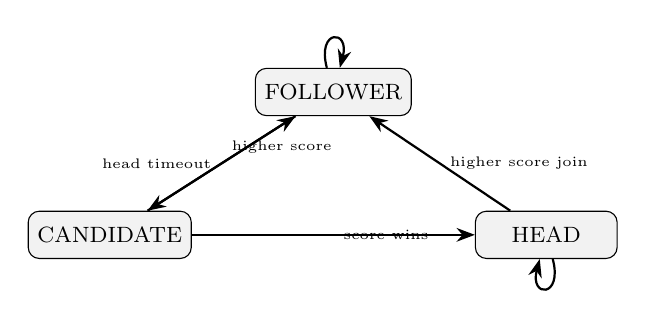
\begin{tikzpicture}[
    font=\footnotesize,
    >=Stealth,
    state/.style={draw, rounded corners, minimum width=1.8cm, minimum height=0.6cm, align=center, fill=gray!10},
    trans/.style={->, thick},
  ]
    \node[state] (follower) {\footnotesize FOLLOWER};
    \node[state, below left=1.2cm and 0.8cm of follower] (candidate) {\footnotesize CANDIDATE};
    \node[state, below right=1.2cm and 0.8cm of follower] (head) {\footnotesize HEAD};
    
    \draw[trans] (follower) -- (candidate) node[midway, left, font=\tiny] {head timeout};
    \draw[trans] (candidate) -- (head) node[midway, right, font=\tiny] {score wins};
    \draw[trans] (candidate) -- (follower) node[midway, above right, font=\tiny] {higher score};
    \draw[trans] (head) -- (follower) node[midway, right, font=\tiny] {higher score join};
    \draw[trans, loop above] (follower) to (follower);
    \draw[trans, loop below] (head) to (head);
  \end{tikzpicture}
  \caption{Cluster-head election FSM. All nodes start as FOLLOWER.
  On head heartbeat timeout, transition to CANDIDATE and broadcast ELECTION.
  If self.score is highest, become HEAD. If a head with higher score appears,
  demote to FOLLOWER.}
  \label{fig:election_fsm}
\end{figure}

\subsection{Submap Transfer FSM (Sender Side)}

\begin{figure}[h]
  \centering
  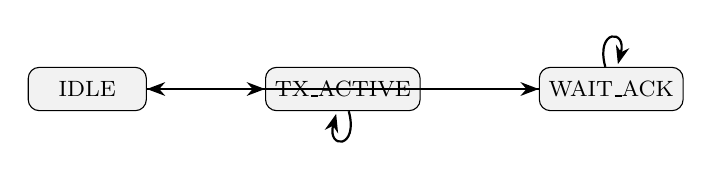
\begin{tikzpicture}[
    font=\footnotesize,
    >=Stealth,
    state/.style={draw, rounded corners, minimum width=1.5cm, minimum height=0.55cm, align=center, fill=gray!10},
    trans/.style={->, thick},
  ]
    \node[state] (idle) {\footnotesize IDLE};
    \node[state, right=1.5cm of idle] (tx) {\footnotesize TX\_ACTIVE};
    \node[state, right=1.5cm of tx] (wait) {\footnotesize WAIT\_ACK};
    
    \draw[trans] (idle) -- (tx);
    \draw[trans] (tx) -- (wait);
    \draw[trans] (wait) -- (idle);
    \draw[trans] (wait) edge[loop above] (wait);
    \draw[trans] (tx) edge[loop below] (tx);
  \end{tikzpicture}
  \caption{Submap transfer FSM (sender side). On SUBMAP\_NACK, re-send missing
  chunks up to 3 times; on 3rd failure, mark submap as failed and notify
  application layer to re-extract at higher compression.}
  \label{fig:submap_fsm}
\end{figure}

\subsection{Connection Lifecycle}

The connection lifecycle has five phases:

\begin{enumerate}
  \item \textbf{Discovery (0--500 ms).} Node broadcasts HELLO with signed
    NodeDescriptor. Existing nodes reply; head sends cluster digest.
  \item \textbf{Calibration handshake (0--2 s).} If $W_i$ unaligned, head sends
    coarse $T_{W_h\leftarrow W_i}$ prior. Refined after first submap exchange.
  \item \textbf{Steady state (indefinite).} POSE\_STREAM at 20 Hz,
    SUBMAP\_PUSH on boundaries, KEYFRAME at 1 Hz, MAP\_DELTA from head at 1 Hz.
  \item \textbf{Autonomous mode (on link loss).} HEARTBEAT timeout over 3 s:
    buffer submaps locally, broadcast HELLO every 1 s. On reconnect, flush
    buffered submaps in chronological order.
  \item \textbf{Leave (on exit).} Send LEAVE; head marks node's submaps as
    owned-but-absent, kept time $T_{\text{keep}}=60$ s, then garbage collected
    unless referenced by loop constraints.
\end{enumerate}

\subsection{Map Consistency Guarantees}

Co-LIC2 provides the following consistency guarantees under the protocol:

\begin{itemize}
  \item \textbf{Monotonic map version.} MAP\_DELTA carries sequential version
    numbers. A member only applies delta $v$ if its local version is $v-1$.
    Lagging members pull full snapshots.
  \item \textbf{Submap idempotency.} Globally unique submap IDs prevent
    duplicate merge. The head maintains a set of recently merged IDs and
    discards duplicates.
  \item \textbf{PGO convergence.} iSAM2 incrementally updates the graph;
    PGO corrections are applied as rigid submap transforms, guaranteeing
    that a submap's internal geometry is preserved.
  \item \textbf{Orphan timeout.} Absent-node submaps are kept for 60 s,
    then garbage collected. If a loop constraint references an orphan
    submap, it is preserved until the constraint is removed.
\end{itemize}


\end{document}
